%%%%%%%%%%%%%%%%%%%%%%%%%%%%%%%%%%%%%%%%%%%%%%%%%%%%%%%%%%%%%%%%%%%%
% Term Extraction as a Filter Framework
%%%%%%%%%%%%%%%%%%%%%%%%%%%%%%%%%%%%%%%%%%%%%%%%%%%%%%%%%%%%%%%%%%%%
\chapter{Information Theoretic and Language Model based Term Extraction using Pointwise Mutual Information}
\chaptermark{Term Extraction using Pointwise Mutual Information}
\label{chap:lmpmi}

This chapter\footnote{Part of the search presented in this thesis has been previously published in \cite{lilingexperttechreport,lilingexpertworkshop}} describes the first main contribution of the thesis, i.e. a novel term extraction technique we have developed based on information theoretic Pointwise Mutual Information (PMI) and language model probabilities. We dub the method $PMI_{LM}$.

The rest of this chapter will first introduce (i) the description of our new monolingual extraction technique, (ii) an intrinsic evaluation of our extraction method against a gold standard terminology, (iii) an extrinsic evaluation of the term extraction in an information retrieval query task and (iv) the bilingual extension of our term extractor based on phrase alignments, iv) an extrinsic evaluation of the automatically extracted bilingual terms on two diverse machine translation tasks.

We show that our monolingual $PMI_{LM}$ term extractor has comparable results with state-of-art term extraction systems in both intrinsic and extrinsic evaluations. Our results of adding terms extracted using the bilingual extension of the $PMI_{LM}$ model agree with previous studies in using additional lexical information in statistical machine translation.

\section{Pointwise Mutual Information}

The Pointwise Mutual Information (PMI) measures the association between two discrete random variables by dividing their joint probability\footnote{i.e. probability of their coincidence} by their individual probabilities\footnote{assuming statistical independence between the variables}. Mathematically,
\vspace{-2mm}
\begin{equation}
\begin{split}
PMI(x,y) & =\log { \frac { p(x,y) }{ p(x)p(y) }  } \\
         & =\log { p(x,y) } -\log { p(x) } -\log { p(y) } 
\end{split}
\end{equation}
\vspace{-2mm}
Applying the chain rule on the PMI equation, we can measure the association between more than two discrete random variables\footnote{See prove on https://en.wikipedia.org/wiki/Pointwise\_mutual\_information\#Chain-rule\_for\_pmi} as such:
\vspace{-2mm}
\begin{equation}
\begin{split}
PMI(xy,z) & =\log { \frac { p(xy,z) }{ p(xy)p(z) }  } \\
& =\log { p(xy,z) } -\log { p(xy) } -\log { p(z) } \\ 
& = PMI(y,z)+PMI(z,y|x) 
\end{split}
\end{equation}
\vspace{-2mm}
In the context of terminology extraction, we can measure the collocation coherence between two words by measuring their PMI \cite{bouma2009normalized,eichler2010dfki}.  For example, to measure the PMI value of the phrase `floating point' 
\vspace{-2mm}
\begin{equation}
\begin{split}
PMI(floating \ point) & =\log { \frac { p(floating \ point) }{ p(floating)p(point) }  } \\
& =\log { p(floating \ point) } -\log { p(floating) } -\log { p(point) } 
\end{split}
\end{equation}
\vspace{-2mm}
where $p(floating,point)$ is the probability of the phrase `\textit{floating point}' divided by the probability of the word `\textit{floating}` and `\textit{point}` occurring individually.

Extending the PMI application to natural text with the chain rule, we can easily find the PMI phrases with more than two words. E.g. for the phrase `\textit{floating point arithmetic}', we can recursively sum the PMI scores of the phrase and the sub-phrases and its sub-phrase.
\vspace{-2mm}
\begin{equation}
\begin{split}
PMI(floating \ point,arithmetic) 
& = \log { p(floating \ point \ arthimetic) } \\
& \quad- \log { p(floating \ point) } -\log { p(arthimetic) } \\ 
% & = pmi(point,arithmetic) + pmi(arithmetic,point|floating) 
\end{split}
\end{equation}

\section{Term Extraction Using Language Model Pointwise Mutual Information}
The calculation of word probabilities and PMI described so far
%in our brief term extraction survey in Chapter 2 
is based on raw counts of a word or term (in Chapter 3 Section 2.5.1). 
$N$-gram language models, that are also based on counts, have developed and applied to other NLP applications such as speech processing and machine translation \citep[e.g.][]{smorgasbord,kirchhoff2005improved,schwenk2012large,lembersky2012adapting,chelba2012distributed}.

A major advantage of using a language model is the possibility of accounting for unknown words using interpolation and smoothing techniques \citep{chen1996empirical,chelba2010}. By using a language model, we avoid the need to optimize n-gram counting when implementing the term extraction algorithm, especially when very fast implementations of language models already exists \citep{kenlm}.

Instead of the using phrasal and word probabilities to compute the PMI score of a term, 

\begin{equation}
PMI(term) = \log { p(w_1,...,w_n) } -\log { p(w_1,...w_{n-1}) } -\log { p(w_n) } 
\end{equation}

we can use a backoff language model as follows:

\begin{equation}
\begin{split}
{ PMI }_{ LM }(term) & = \frac { P_{LM}({ w }_{ 1 },...,{ w }_{ n }) }{ P_{LM}({ w }_{ 1 },...{ ,w }_{ n-1 })P_{LM}({ w }_{ n }) }   \\
& = P_{LM}({ w }_{ 1 },...,{ w }_{ n }) -  P_{LM}({ w }_{ 1 },...,{ w }_{ n-1 }) - P_{LM}({ w }_{ n })
\end{split}
\end{equation}

where a $term$ is made up of words ${ w }_{ 1 },...,{ w }_{ n }$ and $P_{LM}(w)$ is the language model probability provided by a pre-trained language model that approximates to $\log{p(w)}$.

\iffalse
%where ${ PMI }_{ LM }(t)$ is the Pointwise Mutual Information (PMI) score based on language model termhood probability of a term $t$ and $n$ is the total no. of possible $n$-grams (unigrams, bigrams and trigrams) and ${ PMI }_{ LM }({ ngram }_{ i })$ refers to the language model score of the word and its following word. 

%The brevity normalization $1/n$ does not favour a longer term compared to the C-value \citep{frantzi1998c} and the inner context probabilities have either been handled by the $n$-gram model during training or the backoff probability. When an unknown word exists in the term, it uses the backoff probability with the contextual probability of an unknown word occurring in the $w_{i-1}$ and $w_{i-2}$ context.

For example, for the phrase \emph{`floating point arithmetic'} and \emph{`floating point routine'}, we assume that the word \emph{`arithmetic'} is not found in the language model training corpus. Hence the other probabilities were calculated by the language model as follows:

\begin{equation}
{ PMI }_{ LM }('floating \ point \ arithmetic')=1/3! \ *
\left (
\begin{matrix} 
{ P }_{ LM }('floating \ point \ routine') \\
- { P }_{ LM }('floating \ point')
- { P }_{ LM }('point \ routine')
\end{matrix} 
\right )  
\end{equation}

\begin{equation}
{ PMI }_{ LM }('floating \ point \ <UNK>')=1/3! \ *
\left (
\begin{matrix} 
{ P }_{ LM }('floating \ point \ UNK') \\
- { P }_{ LM }('floating \ point')
- { P }_{ LM }('point \ routine')
\end{matrix} 
\right ) 
\end{equation}

\begin{equation}
{ PMI }_{ LM }('floating \ point')=
\begin{matrix} 
{ P }_{ LM }('floating \ point') \\
-({ P }_{ LM }('floating')+{ P }_{ LM }('point'))
\end{matrix} 
\end{equation}

\begin{equation}
{ PMI }_{ LM }('point \ arithmetic')=
\begin{matrix} 
{ P }_{ LM }('point \ UNK') \\
-({ P }_{ LM }('point')+{ P }_{ LM }('UNK')) 
\end{matrix} 
\end{equation}

where ${ P }_{ LM }$ is the language model scores retrieved from the pre-trained trigram language model.
\fi

Similar to the C-value and NC-value \citep{frantzi1998c}, our approach is limited to multi-word expressions. Our approach is (i) a more flexible approach than C-value that allows querying a smoothed language model to retrieve probabilities and (ii) relies on the backoff probabilities that have the ability to score unknown words. The traditional C-value would count co-occurrence instances without smoothed counts and would not handle unknown words. 

%We note that for the single term PMI, we force a PMI value to be isolated from the context where the term occurs. If we use the previous context word before the term, we could get a similar candidate re-ranking as from the NC-value. We did not experiment with the context because we note that finding the correct weights for the C-value and NC-value's cumulative context weight (CCW) should not be as trivial as assigning static 0.2 and 0.8 coefficients in the NC-value calculations. 
%From here on, we refer to our term extraction metric described above as the Language-model PMI ($PMI_{LM}$).

\newpage
\section{Evaluating $PMI_{LM}$ against a Gold Standard}

Intrinsically, we will evaluate the $PMI_{LM}$ against a gold standard terminology in the Biomedical domain. \cite{gurulingappa18empirical} created the \textit{Disease Names and Adverse Effect} (DNAE) corpus with manually annotated medical terms and empirically evaluated a rule-based term extractor, ProMiner, \citep{Hanisch2005}. The ProMiner system uses a pre-processed hand-crafted synonym dictionary to identify potential name occurrences in the biomedical text and associate protein and gene database identifiers with the detected matches. 

\cite{Hanisch2005} considered a subset of the medical terms of the following medical term databases that occurred in the DNAE corpus as the positive examples of the terms that a term extractor should extract. We use the same subset to compare our approach with \cite{Hanisch2005}.

\begin{table}[H]
\centering
    \begin{tabular}{llccc}
    \textbf{System}      & \textbf{Methodology}                 & \textbf{Precision} & \textbf{Recall} &\textbf{ F-score} \\ \hline
    ProMiner    & Unsupervised Rule-based                & \textbf{0.18}      & 0.76   & \textbf{0.29}    \\
    $PMI_{LM}$ (global)     & Unsupervised Probabilistic             & 0.17      &\textbf{ 0.89 }  & \textbf{0.29}    \\ 
    $PMI_{LM}$ (local)     & Unsupervised Probabilistic             & 0.15      &\textbf{ 0.83 }  & 0.25   \\ \hline
    BiOpeNER    & Supervised Off-the-shelf               & \textbf{0.55}      & 0.44   & 0.49    \\
    LM-PMI Linear  & Supervised using Probabilistic Feature & 0.51      & 0.56   & 0.53    \\
    LM-PMI XGBoost  & Supervised using Probabilistic Feature & 0.53      & \textbf{0.58}   & \textbf{0.55 }   \\
    \end{tabular}
\caption{Comparison of $PMI_{LM}$ against State-of-Art Term Extractors}
\label{table:pmllmbiomed}
\end{table}

To directly compare our unsupervised approach (i.e. without the use of the mention annotations from the corpus) against the rule-based ProMiner, we use the $PMI_{LM}$ in two different settings\footnote{Note that the $PMI_{LM}$ approach is limited to multi-word expressions, i.e. ngram orders of two and above. We fall back to the language model probabilities when computing the unigram term scores.} (i) we extracted all possible unigrams to fivegrams from each sentence and filter the top 1200 unique terms weighted by the their 5-gram $PMI_{LM}$ and we search through all documents to label the mentions of these terms, i.e. $PMI_{LM}$ (global) and (ii) we extracted the top 2 unigrams to fivegrams from each sentence and we considered them as the biomedical term that our system identified, i.e. $PMI_{LM}$ (local). Using these two settings, we extracted the terms from the full DNAE corpus and evaluate against the manually annotated terms.

\begin{figure}[!htb]
\centering
	\hspace{-2em}%
	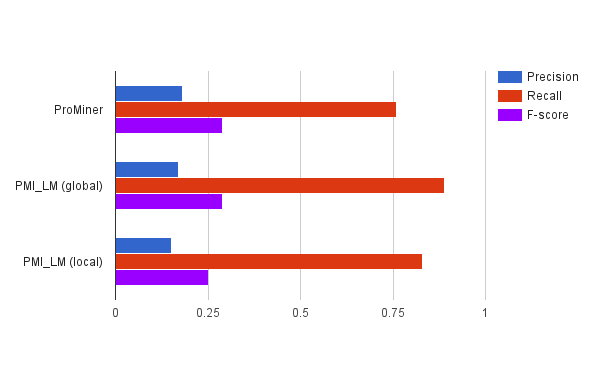
\includegraphics[width=17cm]{unsuper-intrinsic.png} \\[-1em]
	\caption{Precision, Recall and F-score of Unsupervised Term Extraction of $PMI_{LM}$ and ProMiner on the DNAE Corpus}
	\label{fig-unsuper-intrinsic}
\end{figure}

\begin{figure}[!htb]
\centering
	\hspace{-2em}%
	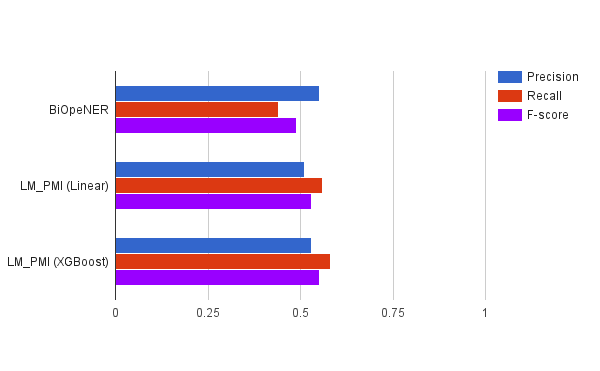
\includegraphics[width=17cm]{super-intrinsic.png} \\[-1em]
	\caption{Precision, Recall and F-score of Supervised Term Extraction of $PMI_{LM}$ and ProMiner on the DNAE Corpus}
	\label{fig-unsuper-intrinsic}
\end{figure}


In the unsupervised scenario, our $PMI_{LM}$ (global) term extractor achieved a similar F-score (0.29) to ProMiner , however our $PMI_{LM}$ (local) system underperformed (F-score=0.25) as compared to ProMiner due to poor precision. This is indirectly caused by the heuristic we impose when extracting the top 2 $PMI_{LM}$ scoring terms per sentence, when in fact there can be 0 or 1 or more than 2 terms within the sentence. 
%In this respect, it reinforces the assumption that salient terms should span across the documents globally and not to every sentence or document. 
On the plus side, we have achieved better recall in both local and global settings at 0.89 and 0.83 respectively as compared to ProMiner that has a recall rate of 0.76.

In a supervised scenario, we use our $PMI_{LM}$ score of all possible ngrams as a sparse feature set to train a linear classifier\footnote{Using the default linear logistic classifier from Scikit-learn\citep{Pedregosa2011}} and an XGBoost ensemble classifier\footnote{Using {\tt hammer.py} wrapper script from \citep{bechara-EtAl:2016:SemEval}. Note that we further slice the 90\% training set to 80\% train and 10\% development to tune the system at every fold for our ensemble system} \citep{chenxgboost} to identify the terms from the manually annotated DNAE corpus. We randomly split the sentences with and 90\% train and 10\% test set and report the harmonic cross-validation precision, recall and F-scores in Table 3.2. We compare our results against the BiOpeNER \citep{biopener} system that also reported harmonic cross-validation scores. 

Although our system did not achieve the state-of-art precision scores that BiOpeNER had, both the linear logistic and ensemble classifier performed better on the recall scores and F-scores. The BiOpeNER system achieved 0.55 precision, 0.44 recall and 0.49 F-score whereas our best setup with the XGBoost achieved 0.53 precision, 0.58 recall and 0.55 F-score.

\section{Evaluating $PMI_{LM}$ in Information Retrieval}

As an extrinsic evaluation, we test the $PMI_{LM}$ term extraction approach on the food domain corpus (WikiFood) that was built for an ontology induction task at SemEval-2015. The corpus contains 869 food terms and the relevant Wikipedia articles that contain these terms. Of those terms 752 terms are multi-words and from the 752 multi-words, we extracted 42,851 sentences (1,207,677 tokens) that contains the multi-word terms. 
%We expect only 1 correct term to be extracted per sentence. 

To access the probabilities for calculating ${ PMI }_{ LM }$, we trained a 5-gram language model on the corpus and we evaluate the ${ PMI }_{ LM }$ accuracy against the traditional C-value score in extracting terms from the corpus. 

We extract the top five term candidates each using ${ PMI }_{ LM }$ and C-value to match against the 1 correct term per sentence. We evaluate the metrics by calculating the accuracy of the top ranked term candidates for each sentence and matching them against the correct term for that sentence. Since the experimental task is structured more like an information retrieval task of candidate ranking, we use the mean reciprocal rank (MRR) to evaluate the ranking efficiency of the term extraction metrics. The mean reciprocal rank is calculated by averaging the ranks of the retrieved candidates against all possible candidates.

\begin{table*}[ht!]
\centering
    \begin{tabular}{l|cc|c}
    ~       & Accuracy (\textit{Top1}) & Accuracy (\textit{Top5}) & MRR   \\ \hline
    \textbf{$PMI_{LM}$}   & \textbf{28.29}           & \textbf{45.18}           & \textbf{1.632} \\
    C-Value & 23.26           & 32.26           & 2.263 \\
    \end{tabular}
\caption{Accuracy and Mean Reciprocal Rank for Term Extraction for WikiFood}
\label{table:pmilmeval}
\end{table*}

Table \ref{table:pmilmeval} presents the results of the experiment on term extraction for the WikiFood Corpus. The $PMI_{LM}$ metric clearly scores better in terms of accuracy to rank the correct term candidate in the top position with a mean rank of 1.63 and an accuracy of 0.28 compared to the C-value’s mean rank of 2.26 and an accuracy of 0.23.

\begin{table*}[ht!]
\centering
    \begin{tabular}{ll|ll}
     \textbf{C-Value}                  & ~      & $PMI_{LM}$                      & ~      \\ \hline
    Bull’s-Eye Barbecue Sauce & -6.491 & Burger King              & -3.269 \\
    Al Steak Sauce            & -7.078 & Bull’s-Eye Barbecue Sauce & -4.909 \\
    Kraft products            & -7.397 & A1 Steak Sauce            & -6.216 \\
    Burger King               & -8.512 & Barbecue Sauce            & -6.304 \\
    A1 Steak                  & -9.148 & Kraft products            & -6.675 \\
    \end{tabular}
    \caption{An Example Output of Ranked Term Candidates and Metrics Scores}
\label{table:pmilmanal}
\end{table*}

However, we do note the low accuracy scores because a term candidate with high termhood might not necessarily be the query term that we are expecting from the sentence. For example in the sentence “\textit{In both cases, Burger King prominently used the names of the Kraft products, A1 Steak Sauce and Bull's-Eye Barbecue Sauce, in the names of the sandwiches}”. The $PMI_{LM}$ and C-value extracted the following terms in Table \ref{table:pmilmanal}.

Although the absolute scores between the two metrics are on a different scale, they are comparable because they are constricted by a probability in the logarithm space. We see that there are many valid terms extracted (e.g. “Burger King” and “Bull’s-Eye Barbecue Sauce”) by both metrics. However, they are not used in the accuracy computation because of the aim to build a food terminology for a taxonomy and to check against a gold standard terminology. 

Unsurprisingly, the C-value favours longer terms and ranks them higher. Additionally, the target “Barbecue Sauce” has been excluded in the top 5 terms for the C-value due to its preference for nested terms and that allowed “A1 Steak” into the top 5 C-value extracted terms.

\section{Bilingual Term Extraction using $PMI_{LM}$}

The discussion until now considers the monolingual term extraction context where the terms are extracted from a single language using the $PMI_{LM}$ scores. Monolingual term extraction revolves around three approaches (i) rule-based methods relying on morphosyntactic patterns, (ii) statistical methods which use association/frequency measures to determine ngrams as MWE and (iii) hybrid approaches that combine rule-based and statistical methods. 

However, where bilingual term extraction techniques are concerned, they operate around two main modus operandi (I) extracting monolingual terms separately and aligning them at word/phrasal level afterwards or (II) aligning parallel text at word/phrasal level and then extracting terms. 

%We proposed a third approach to bilingual extraction without word or phrasal alignments called \texttt{Muwee} \citep{manawi2014} .

%\texttt{Muwee} makes use of the fact that the number of highly collocated MWE should be the same for each sentences pair. \texttt{Muwee} first extracts terms separately from the source and target sentences; the terms are extracted based on bigrams that report Pointwise Mutual Information (PMI) score of above 10. Then for each parallel sentence, if the number of terms are equivalent for the source and target, the bigrams are joined together as a string and contiguous duplicate words are deleted. The removal of contiguous duplicate words is grounded on the fact that linguistically motivated MWE that forms grammatical phrases had shown to improve SMT performances \cite{pal2013impact}.

Given the probabilistic nature of the $PMI_{LM}$, our bilingual term extractor using $PMI_{LM}$ would be language independent. We simultaneously (i) extract the top N terms monolingually for both the source and target languages  and (ii) perform word alignment and phrase extraction to produce a phrase-table using MGIZA++ and Moses \citep{koehn2003statistical,och2003systematic,gao2008parallel}. Then we filter out the terms that do not appear on the phrase table, this will result in a dictionary of aligned terms. 

In this case, we can relate to our bilingual terms as globally extracted like the unsupervised experiment setting in Section 3.1 with the assumption of a top K salient terms ranked by $PMI_{LM}$ that should be added to the training data. 

%Although \texttt{Muwee} does not rely on alignments, we can consider it to be working at a local setting (like in the unsupervised experiment setting in Section 3.1) as it extracts terms per sentence but it is based on the assumption that a threshold exists and it needs to be either empirically tuned or manually set.

\section{Evaluating $PMI_{LM}$ as Additional Lexical Knowledge for SMT}

As a first experiment in integrating terminological information to statistical machine translation, we passively add the bilingually extracted terms, using $PMI_{LM}$ and phrase alignments, to the training data before the phrase-based SMT training process. We use the setup as described in Section 2.4.4. 

We evaluated the integration using the training, development and evaluation data from the Workshop for Asian Translation 2014 (WAT2014) Japanese-English dataset \citep{nakazawa2014overview} from the ASPEC corpus\footnote{http://lotus.kuee.kyoto-u.ac.jp/ASPEC/} \citep{NAKAZAWA16.621}. 

Additionally, we also evaluated the additional $PMI_{LM}$ based lexical knowledge on the Workshop for Machine Translation (WMT14) Russian-English dataset. The development and test set comprises 3000 sentences each from news articles manually translated from English to Russian. The monolingual data consists of News Commentary and News Crawl articles from 2007 to 2014. The training data from WMT15 comprises Common Crawl Corpus, News Commentary, Yandex 1M Corpus and Wiki Headlines Corpus; these were web-crawled texts automatically sentenced aligned.

\begin{table}[H]
\centering
    \begin{tabular}{r|ll|ll}
     \textbf{\#Terms added} & \textbf{EN-JA} & \textbf{JA-EN} & \textbf{EN-RU} & \textbf{RU-EN} \\ \hline
    0                   & 16.75 & \textbf{23.91} & 21.0  & 25.9  \\
    2,000               & 16.68 & 23.74 & 21.6*  & 26.1  \\
    4,000               & 16.67 & 23.79 & 20.9  & 26.0  \\
    6,000               & 16.72 & 23.64 & 21.4  & 26.0  \\
    8,000               & 16.76 & 23.75 & \textbf{22.5*} & 26.7*  \\
    10,000              & \textbf{16.81*} & 23.78 & 22.1*  & 26.5*  \\
    12,000              & 16.59 & 23.45 & 21.4  & \textbf{26.8*}  \\
    \end{tabular}
\caption{BLEU Scores from Phrase-based SMT Systems with Passively Added Terminology of Incremental Sizes; (*) refers to statistically significant results at p $<$ 0.05}
\label{table:pmilmanal}
\end{table}
\vspace{-5mm}
\begin{figure}[!htb]
\centering
	\hspace{-2em}%
	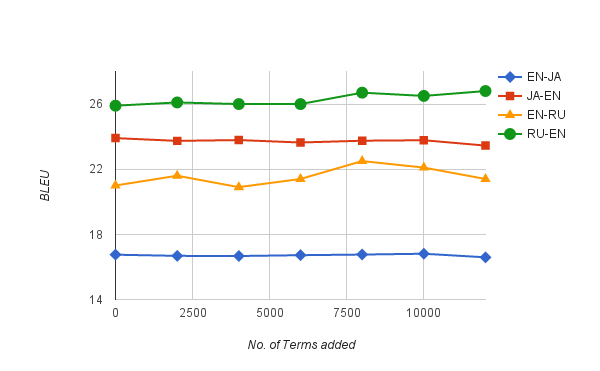
\includegraphics[width=17cm]{num-terms-in-mt.png} \\[-1em]
	\caption{Adding Automatically Extracted Terminology of Different Sizes to SMT}
	\label{fig-numterminmt}
\end{figure}


Table 3.5 and Figure 3.3. presents the results of passively adding varying numbers of  automatically extract bilingual terms to the training data before the statistical machine translation training process. From Table 3.5, we see that adding the top 10,000 bilingual terms to the English-Japanese data yields the highest BLEU score of 16.81 and its statistically significantly (p $<$ 0.05) better than  the baseline system without the added terminology. But this is not the case of the other direction; for Japanese-English, adding the automatically extracted bilingual terminology does not improve upon the baseline but it is also not statistically significantly worse than the baseline.

As for English to Russian, the added terminology performs best (BLEU=22.5) when 8,000 terms are added. In the reverse direction, the BLEU scores can be raised from 25.9 to 26.8 by adding the 12,000 extracted terms.

The results obtain confirms the previous work on adding lexical information to the training set in the attempt of improving machine translation. Most often, previous work as described in Chapter 2 (esp. Section 2.4.3), achieved marginal BLEU gains when passively adding additional lexical information to the training data in a non domain adaptation scenario where the terminology and corpus comes form the same domain.

\section{Summary}

In this chapter, we have proposed a novel information theoretic statistical term extraction technique based on a language model ($PMI_{LM}$) and we have intrinsically and extrinsically evaluated the quality of the terms extracted using the $PMI_{LM}$ based approach.

We show that the $PMI_{LM}$ provides state-of-art performance in extracting biomedical terms in both an unsupervised and a supervised scenario. We have also shown that given the optimal configuration of the automatically extracted terminology and passive integration of the term pairs in statistical machine translation, it is possible to achieve statistically significant though marginal BLEU score improvements.

In Chapter 4, we will describe more experiments to gain insights on how adding manually crafted and automatically extracted dictionary/terminology resource can improve phrased-based statistical machine translation. In the experiments reported in this chapter, ading automatically extracted lexicon passively provides statistically significant but marginal BLEU gains.   



%%%%%%%%%%%%%%%%%%%%%%%%%%%%%%%%%%%%%%%%%%%%%%%%%%%%%%%%%%%%%%%%%%%%
% Using Terminology to Improve Machine Translation
%%%%%%%%%%%%%%%%%%%%%%%%%%%%%%%%%%%%%%%%%%%%%%%%%%%%%%%%%%%%%%%%%%%%
\newpage
\chapter{Using Terminology to Improve Machine Translation}
\label{chap:terminmt}

Phrase-based Statistical Machine Translation (SMT) obtains the best translation by maximizing the conditional probability of the source sentence given the foreign sentence, $p(e|f)$. Using Bayesian deductions, we require the conditional probability of the foreign sentence given the source sentence and the a priori probability of the translation, $p_{LM}(e)$ (Brown, 1993); mathematically

\begin{equation}
arg\max _{  }{ p(e|f)=arg\max _{  }{ p(f|e)\cdot { p }_{ LM }(e) }  } 
\end{equation}


State-of-art SMT systems rely on (i) large bilingual corpora to train the translation model $p(f|e)$ and (ii) monolingual corpora to build the language model, $p_{LM}(e)$ (See Chapter 2, Section 2.2).

There are two primary approaches to the use of bilingual dictionary resources in statistical machine translation: (i) the \textbf{\textit{passive}} approach of appending the parallel training data with a bilingual dictionary and prior to traiing the SMT (ii) the \textbf{\textit{pervasive}} approach of enforcing translation as per the dictionary entries when decoding. 

Previous studies have shown that both approaches of providing external lexical knowledge to statistical machine translation show the potential of improving translation quality (See Chapter 2, Section 2.4.7). In this chapter, empirically investigate the effects of both approaches on the same dataset and provide further insights on how lexical information can be reinforced in statistical machine translation.

The \textbf{\textit{passive}} approach to improve the SMT model is to extend the parallel data with a bilingual dictionary prior to training the model. The primary motivation is to use additional lexical information for domain adaptation to overcome the this issue out-of-vocabulary words during decoding (Koehn and Schroeder, 2007; Meng et al. 2014; Wu et al. 2008). Alternatively, adding in-domain lexicon to parallel data has also shown to carry the potential to improve SMT. The intuition is that by adding extra counts of bilingual lexical entries, the word alignment accuracy improves, resulting in a better translation model (Skadins et al. 2013; Tan and Pal, 2014; Tan and Bond, 2014).

The \textit{\textbf{pervasive}} approach to use a bilingual dictionary is to hijack the decoding process and force word/phrase translations as per the dictionary entries. Previous research used this approach to explore various improvements in industrial and academic translation experiments to enhance specifically term translation consistency.

\section{Passive and Pervasive Lexical Injection}

We view both the passive and the pervasive use of a dictionary in statistical machine translation as a type of lexically constrained statistical MT where in the passive use, the dictionary acts a a supplementary set of bi-lexical rules affecting word and phrase alignments and the resulting translation model and in the pervasive use, the dictionary constraints the decoding search space enforcing translations as per the dictionary entries. 

To examine the \textbf{\textit{passive}} use of a dictionary, we explore the effects of adding the lexicon \textit{n} number of times to the training data until the performance of the machine translation degrades. For the \textbf{\textit{pervasive}} use of a dictionary, we assign a uniform translation probability to possible translations of the source phrase as determined by the dictionary. For instance, in a dictionary, the English term ``\textit{abnormal hemoglobin}” could be translated to 
\begin{CJK*}{UTF8}{min}異常 ヘモグロビン\end{CJK*} or 
\begin{CJK*}{UTF8}{min}異常血色素\end{CJK*}, 
we assign the translation probability of 0.5 to both Japanese translations uniformly, i.e. p(\begin{CJK*}{UTF8}{min}異常 ヘモグロビン\end{CJK*} | abnormal hemoglobin) = p(\begin{CJK*}{UTF8}{min}異常血色素\end{CJK*} | abnormal hemoglobin) = 0.5. If there is only one translation for a term in the dictionary, we force a translation from the dictionary by assigning the translation probability 1.0 to the translation.

One issue with the pervasive use of dictionary translations is the problem of compound phrases in the test sentence that are made up of component phrases in the dictionary. For instance, when decoding the sentence, ``\textit{Here was developed a phase shift \underline{magnetic sensor system} composed of two sets of coils , amplifiers , and phase shifts for sensing and output .}", we fetch the following entries from the dictionary to translate the underlined multiword term:

\begin{itemize}[noitemsep]
\item  magnetic = \begin{CJK*}{UTF8}{min}磁気\end{CJK*}
\item sensor = \begin{CJK*}{UTF8}{min}センサ, センサー, 感知器, 感知部, 感応素子, 検出変換器, 変換素子, 受感部, 感覚器, センサー\end{CJK*}
\item system = \begin{CJK*}{UTF8}{min}組織体制, 制度, 子系, 系列, シス
テム, 体系, 方式, 系統, 秩序, 体制, 組織,
一方式\end{CJK*}
\item  magnetic sensor = \begin{CJK*}{UTF8}{min}磁気センサ\end{CJK*}
\item  sensor system = \begin{CJK*}{UTF8}{min}センサシステム, センサ系, センサーシステム\end{CJK*}
\end{itemize}

In such a situation, where the dictionary does not provide a translation for the complete multi-word string, we set the preference for the dictionary entry with the longest character length in the direction from left to right and select “magnetic sensor” + “system” entries for forced translation. Finally, we investigate the effects of using the bilingual dictionary both passively and pervasively by appending the dictionary before training and hijacking the decoding by forcing translations using the same dictionary.

\subsection{Adding Single Word vs Multi-Word Dictionary Entries to SMT}

Since the phrase-based machine translation model capitalizes on the alignment `consistency’ which essentially requires asymmetric alignment points to extract phrases, it remains unclear whether mono-lexical entries affect the final machine translation quality and how they affect the probability mass during the phrase extraction process. We examine the effects of adding only single word entries vs only adding multi-word entries from the dictionary to the SMT training data to compare the difference between using the full bilingual dictionary vs the mono-lexical or multi-word versions.

% Pikachu, Domosaur, and other Monolexical Languages: http://sigbovik.org/2014/proceedings.pdf

\subsection{Adding a Manually Crafted Dictionary vs an Automatically Extracted Terminology to SMT}

From the literature,\footnote{See Chapter 2 Section 2.3} the popular approach to adding lexical information to statistical machine translation is to passively add automatically extracted a bilingual dictionary / terminology resources to SMT training data. The intrinsic quality of the automatically extracted bilingual dictionary is often disregarded since the ultimate interest is to achieve a BLEU score increment. In the Chapter 3, we experimentally show that both the intrinsic and extrinsic evaluation of the automatically extracted terminology resource using the $PMI_{LM}$ term extraction statistics. 

In the following result section, we would like to explore the difference between using an automatically extracted terminology and a manually crafted dictionary. We use the global $PMI_{LM}$ extraction method described in Chapter 3 to extract the top 100,000 terms to be used as our automatically extracted terminology.

\subsection{Experimental Setup}

We experimented with the passive and pervasive uses of dictionary resources in SMT using the Japanese-English dataset provided in the Workshop for Asian Translation (Toshiaki et al. 2014). We used the Asian Scientific Paper Excerpt Corpus (ASPEC) as the training corpus used in the experiments. The ASPEC corpus consists of 3 million parallel sentences extracted from Japanese-English scientific abstracts from Japan’s Largest Electronic Journal Platform for Academic Societies (J-STAGE). In our experiments we follow the setup of the WAT shared task with 18,00 development and test sentences each from the ASPEC corpus. 

We use the manually crafted Japanese-English (JA-EN) translation dictionaries (JICST, 2004) from the Japan Science and Technology Corporation. It contains 800,000 entries for technical terms manually extracted from scientific and technological documents. 

Similarly, we use the bilingual $PMI_{LM}$ term extractor (from Chapter 3) to extract the top 800,000 terms from the training corpus. We seek to compare the efficacy of the manually crafted dictionary versus the automatically extracted one when using incorporating lexical information in the training data passively and pervasively. 

From Chapter 4.5, in Table 4.5, we note that adding the top 10,000 terms extracted using the $PM_{LM}$ reports statistically significant improvements from the baseline. While the experiment in Chapter 4.5 was concerned about how many unique terms to add to the training data for SMT, the experiments in this chapter using the automatically extracted terms focus on the number of times the extracted terminology is added to the training data for SMT. 

For parity in comparing automatically extracted and manually crafted dictionary resources, we compute the $PMI_{LM}$ values for all entries and extracted the 10,000 terms from the manually crafted dictionary. 

The parallel data, the manually crafted bilingual dictionary and automatically extracted terminology are all tokenized with the MeCab segmenter (Kudo et al. 2004). We use the phrased-based machine translation configuration as described in Chapter 2, Section 2.4.4. 

For the \textit{passive} use of the dictionary, we simply appended the dictionary resources to the training data before the alignment and training process. For the \textit{pervasive} use of the dictionary, we used the {\tt xml-input} function in the Moses toolkit to force lexical knowledge in the decoding process.

Different from the normal use of a dictionary for the purpose of domain adaptation where normally, a domain-specific lexicon is appended to a translation model trained on generic texts, we are investigating the use of an in-domain dictionary in statistical machine translation.

More specifically, we seek to understand how much improvement can be made by skewing the lexical information towards the passive and pervasive use of the dictionary without additional domain knowledge i.e the dictionary comes from the same domain as the training corpus.

\subsection{Results (Passive vs Pervasive)}

\begin{table}[H]
\centering
    \begin{tabular}{l|ll}
    ~           & \textbf{-Pervasive} &\textbf{ +Pervasive }\\ \hline
    \textbf{Baseline}    & 16.75      & 16.87      \\ \hline
    \textbf{Passive x 1 }& 16.83      &  17.30$^{**}$   \\
    \textbf{Passive x 2} & \textbf{17.31$^{**}$}    & 16.87      \\
    \textbf{Passive x 3 }&  17.26$^{*}$    & 17.06      \\
    \textbf{Passive x 4 }& 17.14$^{*}$     &  \textbf{17.38$^{**}$}   \\
    \textbf{Passive x 5 }& 16.82      &  17.29$^{**}$   \\
    \end{tabular}
\caption{BLEU Scores for Passive and Pervasive Use of the Dictionary in SMT (Japanese to English)}
\label{table:hytrajaen}
\end{table}

Table 4.1 presents the BLEU scores of the Japanese to English (JA-EN) translation outputs from the phrase-based SMT system on the WAT test set. The \textbf{-Pervasive} column indicates the number of times a dictionary is appended to the parallel training data (Baseline = 0 times, Passive x$n$ = $n$ time). The \textbf{+Passive} column presents the results from both the passive and pervasive use of dictionary translations, with the exception to the top-right cell which shows the baseline result of the pervasive dictionary usage without appending any dictionary to the training data.

By repeatedly appending the dictionary to the parallel data, the BLEU scores significantly\footnote{*: p-value<0.1, **: p-value<0.001} improves over the baseline from 16.75 to 17.31. Although the system’s performance degrades when adding the dictionary passively thrice, the score remains significantly better than baseline. The pervasive use of the dictionary marginally improves the baseline without the passive use of the dictionary. The best performance is achieved when the dictionary is passively added four times with the pervasive use of the dictionary during decoding.

The small fluctuations in improvement from coupling the passive and pervasive use of an in-domain dictionary give no indication of how both approaches should be used in tandem. However, using either or both the approaches improves the translation quality over the baseline system.

\begin{table}[H]
\centering
    \begin{tabular}{l|ll}
    ~           & \textbf{-Pervasive} &\textbf{ +Pervasive }\\ \hline
    \textbf{Baseline}    & 23.91      & 23.14$^{**}$      \\ \hline
    \textbf{Passive x 1 }& 24.12$^{*}$     &  23.13$^{**}$   \\
    \textbf{Passive x 2} & 23.79    & 22.86$^{**}$      \\
    \textbf{Passive x 3 }&  \textbf{24.14$^{*}$}   & \textbf{23.29$^{**}$}      \\
    \textbf{Passive x 4 }& 24.13$^{*}$     &  23.16$^{**}$   \\
    \textbf{Passive x 5 }& 23.67      &  22.71$^{**}$   \\
    \end{tabular}
\caption{BLEU Scores for Passive and Pervasive Use of the Dictionary in SMT (English to Japanese)}
\label{table:hytraenja}
\end{table}

Table 4.2 presents the BLEU scores of the English to Japanese (EN-JA) translation outputs from the phrase-based SMT system on the WAT test set. The passive use of dictionary outperforms the baseline. Different from the JA-EN translation the pervasive use of dictionary consistently performs worse than the baseline. Upon random manual checking of the MT output, there are many instances where the technical/scientific term in the dictionary is translated correctly with only the passive use of the dictionary. However, it is unclear whether the overall quality of the translations have degraded from the pervasive use of the dictionary given the slight, though significant,\footnote{*: p-value<0.1, **: p-value<0.001} decrease in BLEU scores.

%\vspace{-5mm}
\begin{figure}[!htb]
\centering
	\hspace{-2em}%
	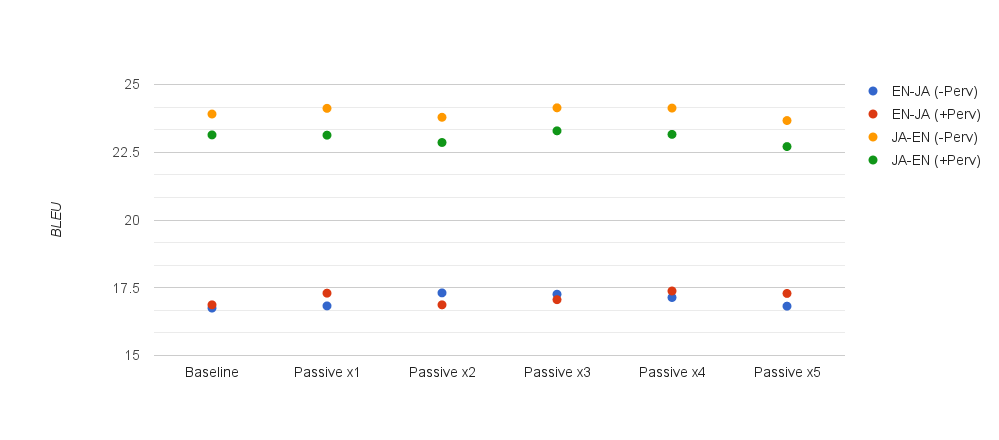
\includegraphics[width=15cm]{hytra.png} \\[-1em]
	\caption{Overview of the Passive and Pervasive Use of Dictionary in the WAT Experiments}
	\label{fig-hytra}
\end{figure}

Figure 4.1 summarizes the results of our experiments on passive and pervasive use of manually created JIST dictionary with the ASPEC corpus evaluated with the WAT evaluation test set. Empirically, both passive and pervasive use of an in-domain dictionary to extend statistical machine translation models with lexical knowledge modestly improve translation quality. Interestingly, the fact that adding the in-domain dictionary information multiple times to the training data improves MT suggests that there may be a critical probability mass by increasing the frequency of in-domain terms which can impact the word and phrasal alignments in a corpus. This may provide insight on optimizing the weights of the salient in-domain phrases in the phrase table.

Although the pervasive use of dictionary information provides minimal or no improvements to the BLEU scores in our experiments, it remains relevant in industrial machine translation where terminological standardization is crucial in ensuring consistent translations of technical manuals or legal texts where incorrect use of terminology may have legal consequences (Porsiel, 2011).

\subsection{Results (Mono-lexeme vs Multi-Word Expressions)}

In a further experiment motivated in Section 4.1.1, we seek to examine the difference between adding mono-lexical entries and multi-word expressions. Table 4.3 presents the results of the experiments on passively adding subsets of the dictionary instead of the full JIST dictionary. The first column (\textbf{Mono-Lexeme}) of Table 4.3 indicates the number of times the mono-lexical entries from the dictionary is appended to the parallel training data (Baseline = 0 times, Passive x1 = 1 time, etc.). The \textbf{Multi-words} column presents the results from adding the multi-word entries from the dictionary to the data before the statistical machine translation training process. The last column of results (\textbf{Full}) in Table 4.3 is the same as the first results column in Table 4.1.

\begin{table}[H]
\centering
    \begin{tabular}{l|lll}
         ~               & \textbf{Mono-Lexeme} & \textbf{Multi-Words} & \textbf{Full} \\ \hline
\textbf{Baseline}        & 16.75      & 16.75      & 16.75  \\ \hline
    \textbf{Passive x1}  & 16.82$^{*}$       & 16.99$^{**}$   & 16.83     \\
    \textbf{Passive x2}  & 16.81$^{*}$       & 16.59     & \textbf{17.31$^{**}$}  \\
    \textbf{Passive x3}  & \textbf{17.01}    & \textbf{17.03}     &  17.26$^{*}$  \\
    \textbf{Passive x4}  & 16.67       & 17.01    & 17.14$^{*}$   \\
    \textbf{Passive x5}  & 16.54       & 16.96    & 16.82   \\
    \end{tabular}
\caption{BLEU Scores in adding Mono-lexeme vs MWE Dictionary to SMT (English to Japanese)}
\label{table:mumtttaenja}
\end{table}

Table 4.3 shows that it is possible to achieve slight statistically significant though marginal improvements from baseline (16.75) by adding the single word once or twice. Adding multi-word entries to the training data also makes statistically significant and marginal improves only when added once. Extending the training data with the full manually crafted dictionary makes the lexical addition more robust and the SMT system makes statistically significant improvements when the dictionary is added 2 to 4 times; the best score (17.31) is achieved when the full dictionary is added twice.

Here we identify a gap in the current strain of research focusing on passively adding only multi-word expressions to SMT training process. Intuitively, we may conjecture that that having mono-lexical entries (e.g. \textit{magnetic = \begin{CJK*}{UTF8}{min}磁気\end{CJK*} sensor = \begin{CJK*}{UTF8}{min}センサ\end{CJK*}; system = \begin{CJK*}{UTF8}{min}シス\end{CJK*}}) that make up the partial multi-word expressions (\textit{magnetic sensor = \begin{CJK*}{UTF8}{min}磁気 センサ\end{CJK*};  sensor system = \begin{CJK*}{UTF8}{min}センサ システム\end{CJK*}}) help in word/phrase alignment process, improving the overall translation quality. But this intuition seems to only hold when translating from English to Japanese. 

\begin{table}[H]
\centering
    \begin{tabular}{l|lll}
         ~               & \textbf{Single Word} & \textbf{Multi-Words} & \textbf{Full} \\ \hline
\textbf{Baseline}        & 23.91      &  23.91      & 23.91  \\ \hline
    \textbf{Passive x1}  & \textbf{23.93}      & 23.96   & 24.12$^{*}$     \\
    \textbf{Passive x2}  & 23.87      & 24.01     & 23.79  \\
    \textbf{Passive x3}  & 23.54   & \textbf{24.14$^{**}$ }    &  \textbf{24.14$^{*}$}  \\
    \textbf{Passive x4}  & 22.91$^{**-}$       & 23.92    & 24.13$^{*}$   \\
    \textbf{Passive x5}  & 23.35       & 23.87$^{**-}$    & 23.67   \\
    \end{tabular}
\caption{BLEU Scores in adding Single Words vs Multi-Words Dictionary to SMT (Japanese to English)}
\label{table:mumtttjaen}
\end{table}

\begin{figure}[H]
\centering
	\hspace{-2em}%
	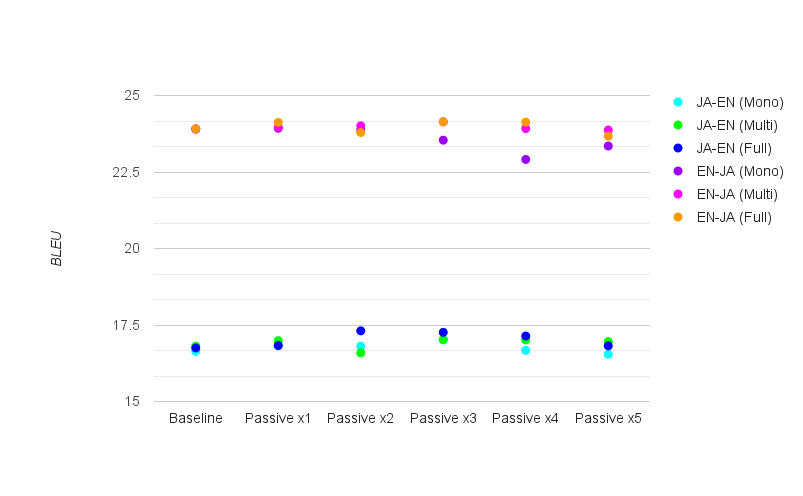
\includegraphics[width=15cm]{mumttt.png} \\[-1em]
	\caption{Overview of the Mono-Lexeme and Mult-Word Expression subset of the Dictionary in the WAT Experiments}
	\label{fig-mumttt}
\end{figure}
\vspace{-5mm}

Table 4.4 compares the results of adding the mono-lexical vs multi-word entries from the dictionary in the attempt to improve BLEU scores\footnote{*: p-value<0.1, **: p-value<0.001}\footnote{*-: p-value<0.1 with negative BLEU from baseline, **-: p-value<0.001 with negative BLEU from baseline}. Interestingly, when translating from Japanese to English, the mono-lexical entries marginally reported lower BLEU scores as compared to the MWEs. And by adding only the multi-word entries, the SMT system achieves similar results to using the full dictionary.

Figure 4.2 summarizes our experiments comparing the addition of mono-lexical and multi-word entries to the statistical machine translation training process. Empirically, we have shown that the usage of the full dictionary might not be necessary depending on the directionality of translation.

\subsection{Results (Manual vs Automatic)}

\begin{table}[H]
\centering
    \begin{tabular}{l|ll|ll}
               & \textbf{JICST} & \textbf{PMI\_LM} & \textbf{JICST} & \textbf{PMI\_LM }  \\ 
                & \textbf{(800k)} & \textbf{(800k)} & \textbf{(10k)} & \textbf{(10k)}  \\ \hline
\textbf{Baseline}  & 16.75 & 16.75 & 16.75 & 16.75 \\ \hline           
                
    \textbf{Passive x1} & 16.83        & 15.34$^{*-}$          & 16.16       & \textbf{16.81}         \\
    \textbf{Passive x2} & \textbf{17.31$^{**}$ }       & 14.82$^{**-}$          & 16.23       & 16.73   \\
    \textbf{Passive x3} & 17.26$^{*}$        & \textbf{15.90$^{*-}$}          & \textbf{16.28}       & 15.68$^{**-}$    \\
   \textbf{Passive x4} & 17.14$^{*}$        & 14.32$^{**-}$          & 15.76$^{*-}$       & 15.54$^{**-}$    \\
    \textbf{Passive x5} & 16.82        & 13.87$^{**-}$          & 15.12$^{*-}$       & 14.91$^{**-}$       
    \end{tabular}
    \caption{BLEU Scores in passively adding a Manually Crafted Dictionary vs an Automatically Extracted Terminology to SMT (English to Japanese)}
\label{table:watlmpmienja}
\end{table}


Table 4.5 shows the result of passively adding a manually crafted dictionary (JICST) against an automatically extracted terminology using $PMI_{LM}$ when translating from English to Japanese. For the comparison that follows, we will keep in mind that our baseline system without adding additional lexical knowledge scores 16.75 BLEU (from Table 4.1) and the significance results\footnote{*: p-value<0.1, **: p-value<0.001}\footnote{*-: p-value<0.1 with negative BLEU from baseline, **-: p-value<0.001 with negative BLEU from baseline} presented on Table 4.5 are with respect to this baseline system.

The \textbf{JICST (800K)} and \textbf{$PMI_{LM}$ (800K)} columns in Table 4.5 shows the results we presented on Table 4.1 when passively adding the full hand-crafted JICST dictionary to the training data and the second column shows the BLEU scores achieved by the same SMT configurations except that we passively add the top 800,000 terms automatically extracted terminology using $PMI_{LM}$. Table 4.5 that all results from passively adding the automatically extracted terms performed significantly worse than the baseline system that scored 16.75 BLEU.

The \textbf{JICST (10K)} and \textbf{$PMI_{LM}$ (10K)}  columns in Table 4.5 present another setting where we added the top 10,000 entries from the manually crafted dictionary ranked by their $PMI_{LM}$ values and an automatically extracted terminology with $PMI_{LM}$ with 10,000 terms. We achieved the best results (16.81 BLEU) when passively adding the automatically extracted terms just once. Although the absolute BLEU score is marginally higher than our baseline (16.75 BLEU), the increment is not significant. Likewise using the smaller subset of the manually crafted dictionary underperforms as compared to using the full dictionary. 

Statistical significance measures the difference of the output of a system from the output of the baseline system. While the negative results of adding automatically extracted terminology are statistically significant, the BLEU score fluctuations are marginal. The overall results did not give a clear signal as to whether adding an automatically extracted dictionary is beneficial or detrimental to the SMT system. 

\begin{figure}[!htb]
\centering
	\hspace{-2em}%
	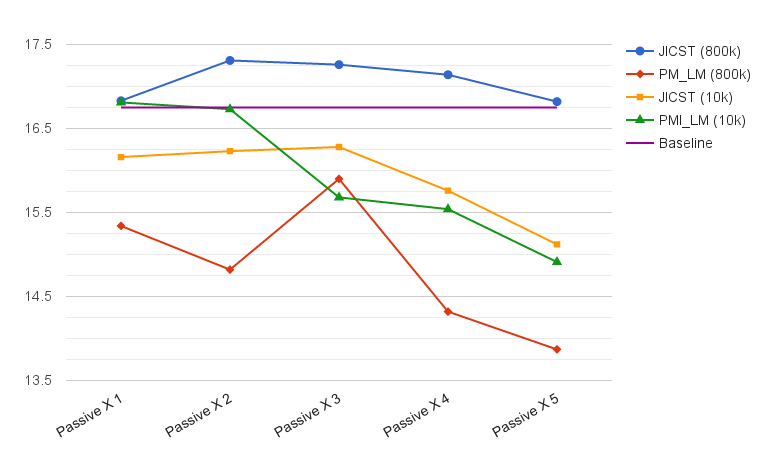
\includegraphics[width=15cm]{dict-term.png} \\[-1em]
	\caption{Passively Adding a Manually Crafted Dictionary vs an Automatically Extracted Terminology (English-Japanese)}
	\label{fig-manvauto}
\end{figure}

Figure 4.3 provides a visual description for Table 4.5. From Figure 4.3, it is more evident that adding the additional lexical information once is optimal when using an automatically extracted terminology (referring to the first green-triangle data point). BLEU scores quickly degrades once we add the 10k terms  more than two times. 

Unsurprisingly, when we filter out the top 10k entries from the manually crafted dictionary, it underperformed as compared to using the full dictionary. However, we see a marginally upwards trend in BLEU scores as we add the dictionary once and twice. This suggests the \textit{`effective multiplier'} idea that (Brown et al., 1993a) proposed\footnote{See Chapter 2, Section 2.3.1}.

The narrative changes when we increase the size of the terminology to 800k, passively adding the automatically extracted terminology thrice performs the best but other than this small anomaly, adding the  terminology follows a linear downwards trend\footnote{Possibly, the fluke in BLEU when passively adding the terminology thrice is caused by the non-deterministic MERT tuning process that found better optimum weights.}. From previous experiments varying the size of the terminology (Chapter 3, Section 3.5), we see that using the top 10,000 terms performed better than 12,000 terms for both English-Japanese and Japanese-English translation\footnote{They are trained and evaluated on the same ASPEC corpus and WAT evaluation dataset}. Thus increasing the size of terminology to 800,000 would just be adding more noise to the system. Interestingly, we see that the phrase-based machine translation is rather robust to the noisy $~$70,000 bilingual terms that we've added and report only slight decrease in BLEU scores. 

\begin{table}[H]
\centering
    \begin{tabular}{l|ll|ll}
               & \textbf{JICST} & \textbf{PMI\_LM} & \textbf{JICST} & \textbf{PMI\_LM} \\ 
               & \textbf{(800k)} & \textbf{(800k)} & \textbf{(10k)} & \textbf{(10k)} \\ \hline
 \textbf{Baseline}  & 23.91 &23.91  & 23.91 & 23.91 \\ \hline
    \textbf{Passive x1} & 24.12$^{*}$        & 23.26$^{*-}$          & \textbf{23.85}       & \textbf{23.78}        \\
   \textbf{Passive x2} & 23.79        & \textbf{23.45}          & 23.72       & 23.76      \\
    \textbf{Passive x3} & \textbf{24.14$^{*}$ }       & 22.81$^{*-}$          & 22.84$^{*-}$       & 22.93$^{*-}$       \\
    \textbf{Passive x4} & 24.13$^{*}$        & 22.35$^{*-}$          & 23.04$^{*-}$       & 23.01$^{*-}$         \\
    \textbf{Passive x5} & 23.67        & 21.93$^{*-}$          & 22.91$^{*-}$       & 23.00$^{*-}$   
    \end{tabular}
    \caption{BLEU Scores in adding Manually Crafted Dictionary vs Automatically Extracted Terminology to SMT (Japanese to English)}
\label{table:watlmpmijaen}
\end{table}

Table 4.6 shows the result of passively adding a manually crafted dictionary (JICST) against an automatically extracted terminology using $PMI_{LM}$ when translating from Japanese to English. For the comparison that follows, we will bear in mind that our baseline system without adding additional lexical knowledge scores 23.91 BLEU (from Table 4.2) and the presented on Table 4.5 are respectively to this baseline system.

\vspace{-5mm}
\begin{figure}[!htb]
\centering
	\hspace{-2em}%
	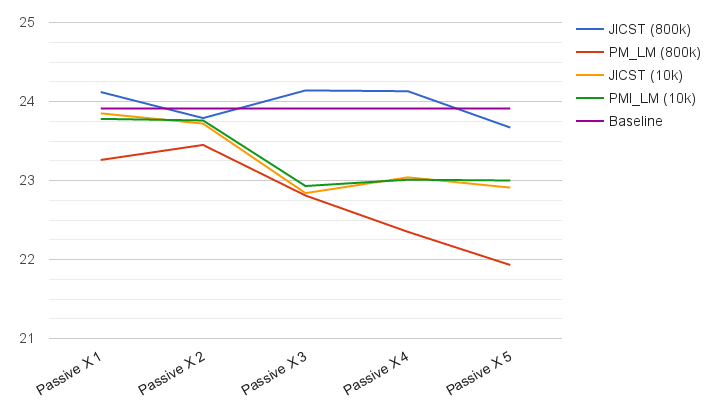
\includegraphics[width=15cm]{term-dict.png} \\[-1em]
	\caption{Passively Adding Manually Crafted Dictionary vs Automatically Extracted Terminology (Japanese-English)}
	\label{fig-manvauto}
\end{figure}

Figure 4.4 presents the results better graphically. similar to translating from English to Japanese, the best performance is achieved by passively adding manually crafted dictionary (BLEU 24.14), in this case adding it thrice. We see the same robustness of the SMT system given the noisy lexical information as the BLEU score drops marginally though the deterioration is statistically significant. 

In contrast to passively adding 800k automatically extracted terms  when translation from EN-JA, we see a slight increase in BLEU 23.26 -> 23.45  when the 800k terms were added twice. However, the same linearly degenerate behavior happens as we continue to passively increase the effective multiplier. 

As we reduce to the automatically extracted terminology size and the manually crafted dictionary size to 10k, we see that we achieved better results but still lower than the baseline (23.91 BLEU). But this does not come as a surprise since the best possible results from adding lexical information comes from adding the full JICST dictionary and it scantily improves upon the baseline system 23.91 -> 24.14.

\section{Summary}

In this chapter, we explore the multiple facade to integrate lexical information to phrase-based statistical machine translation  from (i) comparing passive and pervasive techniques, to understanding (ii) the synergy in using both mono-lexical and multi-word entries in passively adding lexicon to the SMT process and (iii) the difference in adding manually crafted versus automatically extracted lexicon to the SMT training data. 

In general, passively adding additional lexical information to statistical machine translation performs better than pervasively forcing the machine translation decoder to use the bilingual lexicon entries. To achieve optimal `effective multiplier' effect in passively addition lexicon to machine translation, we found that adding the lexicon more than once improves the performance; in our experiments, we found that adding 3-4 times yields the best result. Additionally, adding manually crafted dictionaries outperforms automatically extracted dictionaries. 



\iffalse
\section{Experiments on Workshop for Machine Translation (WMT) Dataset}
    \subsection{Using Named Entities and MWE for EN-HI Translations}
    \subsection{Using JRC Named Entities for EN-RU Translations}
\fi
    


%%%%%%%%%%%%%%%%%%%%%%%%%%%%%%%%%%%%%%%%%%%%%%%%%%%%%%%%%%%%%%%%%%%%
% Other Techniques to Improve Machine Translation
%%%%%%%%%%%%%%%%%%%%%%%%%%%%%%%%%%%%%%%%%%%%%%%%%%%%%%%%%%%%%%%%%%%%

\chapter{Measuring the Goodness of Machine Translation}
%\chapter{Measuring Goodness of Machine Translation}
\label{chap:goodness}

The discussion up till now on evaluating  translation quality is based on BLEU scores (Papineni et al., 2002) and its statistical significance based on bootstrap resampling  (Koehn, 2004). In this Chapter, we propose a different way to look at machine translation evaluation focusing on (i) evaluating the semantic `goodness' of machine translated texts by casting it as a semantic textual similarity task and (ii) highlighting an awkward disparity between BLEU / RIBES\footnote{An extension of BLEU} and human evaluation of translated text. 

\newpage
\section{Evaluating Semantic `Goodness' of Machine Translated Texts}

Translation is becoming an utility in everyday life. The increased availability of real-time machine translation services relying on Statistical Machine Translation (SMT) allows users who do not understand the language of the source text to quickly gist text in a foreign language and understand its general meaning. For these users, often the accurate meaning of translated words is more important than the fluency of the translated sentence.

However, SMT can suffer from poor lexical choices. Fluent but inadequate translations are commonly produced due to the strong bias towards the language model component that prefers consecutive words based on the data that the system is trained on.

Current state of art MT evaluation metrics are generally able to identify problems with the grammaticality of the translation but less evidently the accuracy of translated semantics, e.g. incorrect translation of ambiguous words or wrong assignment of semantic roles. In the example below, the ideal Machine Translation (MT) evaluation metric should appropriately penalise poor lexical choice, such as `\textit{braked}', and reward or at least allow leeway for semantically similar translations, such as `\textit{external trade}'.

\begin{itemize}[noitemsep]
\item[] \textbf{Source (DE):} 
\item[] \textit{Auch der Aussenhandel bremste die Konjunktur.} 
\item[] \textbf{Phrase-based MT:} 
\item[] \textit{The foreign trade braked the economy.}
\item[] \textbf{Neural MT:} 
\item[] \textit{External trade also slowed the economy.}
\item[] \textbf{Reference (EN):} 
\item[] \textit{Foreign goods trade had slowed, too.}
\end{itemize}

The German word \textit{bremste} is commonly used as `\textit{braked}' in the context of driving, but the appropriate translation should have been `\textit{slowed}' in the example mentioned above. Although the phrase \textit{external trade} differs from f\textit{oreign goods trade} in the reference sentence, it should be considered as an acceptable translation.

To pursue a semantically motivated measure of goodness for machine translation, we pursue an evaluation metric that takes into account both fluency (grammaticality) and adequacy (semantics) to evaluate whether the machine translation output has the same meaning as its reference translation through the Semantic Textual Similarity (STS) task. Semantic Textual Similarity (STS) is the task of measuring the degree to which two texts have the same meaning \citep{Agirre2014}.  For instance, given the two texts,  ``\emph{the man is slicing the tape from the box.}" and ``\emph{a man is cutting open a box.}", an STS system predicts a real number similarity score on a scale of 0 (no relation) to 5 (semantic equivalence). In this case we can relate the pair of texts closely to what we are evaluating when measuring the goodness of machine translation output if we treat one of the sentence as the output and the other as the reference.

We propose a model that approaches the task by (i) combining existing machine translation evaluation metrics (that are good in determining fluency) and (ii) using linguistically motivated monolingual word alignments and neural embeddings (to add the semantic dimension to our new metric). We call our metric, {\tt Stasis}.\footnote{Part of the research in this chapter has been published in \cite{usaarsheff2015,usaarsheff2016}}

\subsection{Measuing Grammatical Fluency with MT Evaluation Metrics Ensemble}

Previous approaches have applied MT evaluation metrics for the STS task with progressively improving results \citep{Agirre2012,Agirre2013,Agirre2014,agirre2015}. We propose a single MT evaluation metric by ensembling a glut of MT evaluation metrics.\footnote{This section presents a collaborative work between Saarland University and University of Sheffield\footnote{A partner institute in the EXPERT project} in developing the MT evaluation metric ensemble.} 

\subsubsection{Previous Usage of MT Metrics to Determine Textual Similarity}
At the pilot English STS-2012 task, \cite{Rios2012} trained a Support Vector Regressor using the lexical overlaps between the surface strings, named entities and semantic role labels and the BLEU \citep{Papineni2002} and METEOR \citep{Banerjee2005,Denkowski2010} scores between the text snippets and their best system scored a Pearson correlation mean of 0.3825. The system underperformed compared to the organizers' baseline system\footnote{Refers to the token cosine baseline system ({\tt baseline-tokencos}) in STS-2012.} which scored 0.4356. 

For the English STS-2013 task, \cite{Barron-Cedeno2013} also used a Support Vector Regressor with an larger array of machine translation metrics (BLEU, METEOR, ROUGE \citep{lin-och:2004:ACL}, NIST \citep{doddington2002automatic}, TER \citep{snover2006study}) with measures that compute similarities of dependency and constituency parses \citep{liu2005syntactic} and semantic roles, discourse representation and explicit semantic analysis \citep{gabrilovich2007computing} annotations of the text snippets. These similarity measures are packaged in the Asiya toolkit \citep{Gimenez2010}. They scored 0.4037 mean score and performed better than the Takelab baseline \citep{vsaric2012takelab} at 0.3639.

At the SemEval-2014 Cross-level Semantic Similarity task \citep{jurgens2014crosssts,Jurgens2015}, participating teams submitted similarity scores for text of different granularity. \cite{Huang2014} used a linear regressor solely with MT evaluation metrics (BLEU, METEOR, ROUGE) to compute the similarity scores between  paragraphs and sentences. They scored 0.792 beating the lowest common substring baseline which scored 0.613.

In the SemEval-2015 English STS and Twitter similarity tasks, \citep{berterofung2015} trained a neural network classifier using (i) lexical similarity features based on WordNet \citep{miller1995wordnet}, (ii) neural auto-encoders \citep{socher2011dynamic}, syntactic features based on parse tree edit distance \citep{zhang1989simple,wan2006using} and (iii) MT evaluation metrics, viz. BLEU, TER, SEPIA \citep{habash2008sepia}, BADGER \citep{parker2008badger} and MEANT \citep{lo2012fully}.

For the classic English STS task in SemEval-2015, \cite{usaarsheff2015} used a range of MT evaluation metrics based on lexical (surface $n$-gram overlaps), syntactic (shallow parsing similarity) and semantic features (METEOR variants) to train a Bayesian ridge regressor. Their best system achieved 0.7275 mean Pearson correlation outperforming the {\tt token-cos} baseline which scored 0.5871 while the top system \citep{sultan2015} achieved 0.8015.

Another notable mention of MT technology in the STS tasks is the use of referential translation machines to predict and derive features instead of using MT evaluation metrics \citep{Bicici2013,Bicici2014,bicici2015}.

\subsubsection{Feature Matrix}

Following the success of STS systems that use MT evaluation metrics, we train three regression models using an array of MT metrics based on lexical, syntactic and semantic features. 

Machine translation evaluation metrics utilize various degrees of lexical, syntactic and semantic information. Each metric considers several features that compute the translation quality by comparing a translation against one or several reference translations. 

We trained our system using the follow feature sets: (i) $n$-gram, shallow parsing and named entity overlaps ({\tt Asiya}), (ii) {\tt BEER}, (iii) {\tt METEOR} and (iv) {\tt ReVal}. Although {\tt BEER} and {\tt METEOR} metrics provided mecahnisms to fine-tuned the metric with respect to the training data, we did not tune these metrics because they will be used as input features that will be fed into an ensemble which will automatically learn their feature weights which effectively fine-tuned the metric to the training data too. 

\textbf{{\tt Asiya} Features}: \cite{gonzalez2014} introduced a range of language independent metrics relying on $n$-gram overlaps similar to the modified $n-$-gram precisions of the BLEU metric \citep{Papineni2002}. Different from BLEU, \cite{gonzalez2014} computes $n$-gram overlaps using similarity coefficients instead of proportions. We use the {\tt Asiya} toolkit \citep{Gimenez2010} to annotate the dataset with the similarity coefficients of $n$-gram overlap features described in this section. We use 16 features from both cosine similarity and Jaccard Index coefficients of the character-level and token-level $n$-grams from the order of bigrams to 5-grams. Additionally, we use the Jaccard similarity of the pseudo-cognates and the ratio of $n$-gram length as the 17th and 18th features. Adding a syntactic dimension to our feature set, we use 52 shallow parsing features described in \cite{usaarsheff2015}; they measure the similarity coefficients from the $n$-gram overlaps of the lexicalized shallow parsing (aka chunking) annotations. As for semantics, we use 44 similarity coefficients from Named Entity (NE) annotation overlaps between two texts. After some feature analysis, we found that 22 out of the 44 NE $n$-gram overlap features and 1 of the shallow parsing features have extremely low variance across all sentence pairs in the training data. We removed these features before training our models.

\textbf{{\tt BEER} Features}: \cite{stanojevic2014beer} presents an MT evaluation metric that uses character $n$-gram overlaps, the Kendall tau distance of the monotonic word order \citep{isozaki2010automatic,birch2010lrscore} and abstract ordering patterns from tree factorization of permutations \citep{zhang2007factorization}. While Asiya features are agnostic to word classes, BEER differentiates between function words and non-function words when calculating its adequacy features. 

\textbf{{\tt METEOR} Features}: METEOR first aligns the translation to its reference, then it uses the unigram mapping to see whether they match based on their surface forms, word stems, synonyms and paraphrases \citep{Banerjee2005,Denkowski2010}. Similar to BEER features, METEOR makes a distinction between content words and function words and its recall mechanism weights them differently. We use all four variants of METEOR: exact, stem, synonym and paraphrase. 

\textbf{{\tt ReVal} Features}: ReVal \citep{reval2015} is a deep neural net based metric which uses the cosine similarity score between the Tree-based Long Short Term Memory (LSTM) \citep{hochreiter1997long,cho2014,treelstm} dense vector space representations of two sentences.

\subsubsection{The MT Metric Ensemble}

The STS 2012 to 2015 datasets are made up of sentence pairs with manually annotated scores of the similarity between each pair of sentences. We annotated the STS 2012 to 2015 datasets with the features as described in the previous section and trained three models using (i) a linear regressor ({\tt Linear}), (ii) boosted tree regressor ({\tt Boosted}) \citep{friedman2001greedy} and (iii) eXtreme Gradient Boosted tree regressor ({\tt XGBoost}) \citep{chen2015xgboost,chenxgboost}.

%%%%%%%%%%%%%%%%%%%%%%%%%%%%%%%%%%%%%%%%%%%%%%%%%%%%%%%%%%%%%%%%%%

\subsection{Measuing Semantic Adequacy With Monolingual Word Alignments and Neural Network Embeddings}

For the 2014 and 2015 editions of the STS task, the top performing submissions are from the DLS@CU team \citep{sultan2014dls,sultan2015dls}. 

Their STS2014 submission is based on the proportion of overlapping content words between the two sentences treating semantic similarity as a monotonically increasing function of the degree to which two sentences contain semantically similar units and these units occur in similar semantic contexts \citep{sultan2014dls}. Essentially, their semantic metric is based on the proportion of aligned content words between two sentences, formally defined as:

\vspace{-2mm}

\begin{equation}\label{eq:prop-al}
{ prop }_{ Al }^{ (1) }=\frac { |\{ i:[\exists j:(i,j)\in Al] \ and \ { w }_{ i }^{ (1) }\in C\} | }{ |\{ i:{ w }_{ i }^{ (1) }\in C\} | } 
\end{equation}

where ${ prop }_{ Al }^{ (1) }$ is the monotonic proportion of the semantic unit alignment from a set of alignments $Al$ that maps the positions of the words $(i,j)$ between sentences $S^{(1)}$ and $S^{(2)}$, given that the aligned units belong to a set of content words, $C$. Since the proportion is monotonic, the equation above only provides the proportion of semantic unit alignments for $S^{(1)}$. The $Al$ alignments pairs are automatically annotated by a monolingual word aligner \citep{sultan2014back} that uses word similarity measures based on contextual evidence from the Paraphrase Database (PPDB) \citep{ppdb} and syntactic dependencies.

The same computation needs to be made for $S^{(2)}$. An easier formulation of Equation \eqref{eq:prop-al} without the formal logic symbols is:

\vspace{-5mm}

\begin{equation}\label{eq:prop-al-pythonic}
{ prop }_{ Al }^{ (1) }=\frac { sum(1 \ for \ { w }_{ i },{ w }_{ j } \ in \ { Al }^{ (1,2) } \ if \ { w }_{ i } \ in \ C) }{ sum(1 \ for \ { w }_{ i } \ in \ { S }^{ (1) } \ if \ { w }_{ i } \ in \ C) } 
\end{equation}

\vspace{2mm}

Since the semantic similarity between  $(S^{(1)}, S^{(2)})$ should be a single real number, \cite{sultan2014dls} combined the proportions using harmonic mean:

\vspace{-5mm}

\begin{equation}\label{eq:sim-sent}
sim({ S }_{  }^{ (1) },{ S }_{  }^{ (2) })=\frac { 2*{ prop }_{ Al }^{ (1) }*{ prop }_{ Al }^{ (2) } }{ { prop }_{ Al }^{ (1) }+{ prop }_{ Al }^{ (2) } } 
\end{equation}

Instead of simply using the alignment proportions, \cite{sultan2015dls} extended their hypothesis by leveraging pre-trained neural net embeddings \citep{baroni2014composes}. \cite{sultan2015dls}  posited that the semantics of the sentence can be captured by the centroid of its content words\footnote{In the implementation, they have used lemmas instead of words to reduce sparsity when looking up the pre-trained embeddings (personal communication with Arafat Sultan).} computed by the element-wise sum of the content word embeddings normalized by the number of content words in the sentence. Together with the similarity scores from Equation \eqref{eq:sim-sent} and the cosine similarity between two sentence embeddings, \cite{sultan2015dls} trained a Bayesian ridge regressor to learn the similarity scores between text snippets. 

\subsubsection{Replicating of DLS}

To replicate the success of \cite{sultan2014dls}, we use the monolingual word aligner from \cite{sultan2014back} to annotate the STS-2012 to STS-2015 datasets and computed the alignment proportions as in Equation \eqref{eq:prop-al} and \eqref{eq:prop-al-pythonic}.

In duplicating \cite{sultan2015dls} work, we first have to tokenize and lemmatize text. The details of pre-processing choices was undocumented in their paper, thus we lemmatized the datasets with the NLTK tokenizer \citep{bird2009natural} and PyWSD lemmatizer \citep{pywsd14}. We use the lemmas to retrieve the word embeddings from the COMPOSES vector space \citep{baroni2014composes}. Similar to Equation \eqref{eq:prop-al-pythonic} (changing only the numerator), we sum the sentence embedding's centroid as follows:

\vspace{-5mm}

\begin{equation}
v(S_{  }^{ (1) })=\frac { sum(v({ w }_{ i }) \ for \ { w }_{ i } \ in  \ { S }^{ (1) } \  if \ { w }_{ i } \ in  \ C) }{ sum(1 \ for \ { w }_{ i } \ in \ { S }^{ (1) } \ if \ { w }_{ i } \ in \ C) } 
\end{equation}

where $v(S_{  }^{ (1) })$ refers to the dense vector space representation of the sentence $S_{  }^{ (1) }$ and $v({ w }_{ i })$ refers to the word embedding of word $i$ provided by the COMPOSES vector space. The same computation has to be done for $S_{  }^{ (2) }$.

Intuitively, if either of the sentences contains more or less content words than the other, we can see the numerator changing but the denominator changes with it. The difference between $v(S_{  }^{ (1) })$ and $v(S_{  }^{ (2) })$ contributes to \emph{distributional semantic distance}. 

To calculate a real value similarity score between the sentence vectors, we take the dot product between the vectors to compute the cosine similarity between the sentence vectors:

\vspace{-2mm}

\begin{equation}
sim({ S }_{  }^{ (1) },{ S }_{  }^{ (2) })=\frac { v(S_{  }^{ (1) })\cdot v(S_{  }^{ (2) }) }{ |v(S_{  }^{ (1) })| \ |v(S_{  }^{ (2) })|  } 
\end{equation}

There was no clear indication of which vector space \cite{sultan2015dls} have chosen to compute the similarity score from Equation 5.5. Thus we compute two similarity scores using both COMPOSES vector spaces trained with these configurations:

\begin{itemize}
\item 5-word context window, 10 negative samples, subsampling, 400 dimensions
\item 2-word context window, PMI weighting, no compression, 300K dimensions
\end{itemize}

In this way, we extracted two similarity features for every sentence pair. With the harmonic proportion feature from Equation 5.3 and the similarity scores from Equation 5.5, we trained a boosted tree ensemble on the 3 features using the STS 2012 to 2015 datasets and submitted the outputs from this model as our baseline submission in the English STS Task in SemEval 2016. 

\subsubsection{Replacing COMPOSES with GloVe}

\cite{glove2014} handles semantic regularities \citep{levy2014linguistic} explicitly  by using a global log-bilinear regression model which combines the global matrix factorization and the local context vectors when training word embeddings.

Instead of using the COMPOSES vector space, we experimented with replacing the  $v({ w }_{ i })$ component in Equation 5.4 with the GloVe vectors,\footnote{We use the 300 dimensions vectors from the GloVe model trained on the Commoncrawl Corpus with 840B tokens, 2.2M vocabulary.} $v_{glove}({ w }_{ i })$ such that:

\vspace{-5mm}

\begin{equation}
sim_{glove}({ S }_{  }^{ (1) },{ S }_{  }^{ (2) })=\frac { v_{glove}(S_{  }^{ (1) })\cdot v_{glove}(S_{  }^{ (2) }) }{ |v_{glove}(S_{  }^{ (1) })| \ |v_{glove}(S_{  }^{ (2) })|  } 
\end{equation}

\vspace{2mm}

The novelty lies in the usage of the global matrix to capture corpus wide phenomena that might not be captured by the local context window. The model leverages on both the non-zero elements in the word-word co-occurence matrix (not a sparse bag-of-words matrix) and the individual context window vectors similar to the word2vec model \citep{mikolov2013distributed}. 

\subsubsection{Similarity Using Tree LSTM}
Recurrent Neural Nets (RNNs) allow arbitrarily sized sentence lengths \citep{elman1990finding} but early work on RNNs suffered from the vanishing/exploding gradients problem \citep{bengio1994learning}. \cite{hochreiter1997long} introduced multiplicative input and output gate units to solve the vanishing gradients problem. While RNN and LSTM process sentences in a sequential manner, Tree-LSTM extends the LSTM architecture by processing the input sentence through a syntactic structure of the sentence. We use the ReVal metric \citep{reval2015} implementation of Tree-LSTM \citep{tai-socher-manning:2015}  to generate the similarity score.

ReVal represents both sentences ($h_{1}$, $h_{2}$) using Tree-LSTMs and predicts a similarity score $\hat{y}$ based on a neural network which considers both distance and angle between $h_{1}$ and $h_{2}$:

\begin{equation}
%\begin{align}
\label{eq2}
\begin{split}
h_{\times} & =h_{1}\odot h_{2}
\\ 
h_+ & =|h_{1}-h_{2}| 
\\
h_s & =\sigma\left(W^{(\times)}h_{\times} + W^{(+)}h_+ +b^{(h)}\right)
\\
\hat{p}_{\theta} & = \text{softmax} \left(W^{(p)}h_s + b^{(p)}\right)
\\
\hat{y} & =r^T\hat{p}_{\theta}
\end{split}
%\end{align}
\end{equation}
where, $\sigma$ is a sigmoid function, $\hat{p}_\theta$ is the estimated probability distribution vector and $r^T=[1$ $2 ... K]$. 
The cost function $J(\theta)$ is defined over probability distributions $p$ and $\hat{p}_{\theta}$  using regularised Kullback–Leibler (KL) divergence. 
\begin{equation}
\label{eq3}
J(\theta)  = \frac{1}{n} \sum_{i=1}^{n} \text{KL}\left(p^{(i)}\middle|\middle|\hat{p}_{\theta}^{(i)}\right) + \frac{\lambda}{2}{||\theta||}_2^2
\end{equation}
In Equation \ref{eq3}, $i$ represents the index of each training pair, $n$ is the number of training pairs and $p$ is the sparse target distribution such that $y=r^Tp$ is defined as follows:
\[
    p_j= 
\begin{cases}
    y- \lfloor{y\rfloor},& j = \lfloor{y\rfloor} + 1\\
    \lfloor{y\rfloor} -y +1, & j = \lfloor{y\rfloor}\\
    0              & \text{otherwise}
\end{cases}
\]
for $1\le j \le K$, where, $y\in[1, K]$ is the similarity score of a training pair. This gives us a similarity score between [1, K] which is mapped to [0, 1].\footnote{score = (score-1)/K Please refer to \cite{reval2015} for training details.}

\subsubsection{A Semantically Adequate Metric}

Similar to our approach in the MT metric ensemble, we annotated the STS 2012 to 2015 datasets with the semantic similarity features as described in the previous section and trained three models using (i) a linear ridge regressor ({\tt L}) that uses the similarity score from Equations 6.3 and 6.5 as features, (ii) extending the linear regression, we included the similarity score from Equations 6.6 and 6.8 to the feature set and trained a boosted tree ensemble \citep{friedman2001greedy} ({\tt B}) (iii) we use the same feature set as our B system to train an eXtreme Gradient Boosted tree regressor ({\tt XGBoost}) \citep{chen2015xgboost,chenxgboost}, we refer to it as ({\tt X}).

\subsection{Experimental Setup and Results}

We evaluated the two components of our {\tt Stasis} metric using the STS2016 dataset that consist of text snippets from the following domains, (i) forum answers, (ii) forum questions, (iii) news headlines, (iv) plagiarism checking samples from student essays and (v) post-editing texts.

\begin{table}[H]
\centering
    \begin{tabular}{l|ccccc|c}
            & answer-answer & headlines & plagiarism & postediting & question-question & Overall     \\ \hline
    {\tt MT Ensemble (L)}  & 0.31539       & 0.76551   & 0.82063    & 0.83329     & \textbf{0.73987}           & 0.68923 \\
    {\tt MT Ensemble (B)} & 0.37717       & 0.77183   & 0.81529    & 0.84528     & 0.66825           & 0.69259 \\
    {\tt MT Ensemble (X)} & \textit{0.47716} & \textbf{0.78848} & \textbf{0.83212}    & \textit{0.84960}      & 0.69815           & \textit{0.72693} \\ \hline
   {\tt Semantic (L)} & 0.48799       & 0.71043   & 0.80605    & 0.84601     & 0.61515           & 0.69244 \\
    {\tt Semantic (B)}  & 0.49415       & 0.71439   &\textit{ 0.79655 }   & 0.83758     & \textit{0.63509 }          & 0.69453 \\
    {\tt Semantic (X)}  & \textit{0.49947 }      & \textit{0.72410 }   & 0.79076    & \textit{0.84093}     & 0.62055           & \textit{0.69471} \\ \hline
\textbf{{\tt Stasis (X)}} & \textbf{0.50628} &  0.77824 & 0.82501 &  \textbf{0.84861} & 0.70424 & \textbf{0.73050} \\ \hline
Median & 0.48018 & 0.76439 & 0.78949 & 0.81241 & 0.57140 & 0.68923 \\
Best & 0.69235 & 0.82749 & 0.84138 & 0.86690 & 0.74705 & 0.77807 \\
    \end{tabular}
\caption{{\tt Stasis} Metric Evaluated on the STS-2016 Task;  \textit{Best} is the best performing results per domain from various systems participating in the English STS-2016 shared task and \textit{Median} is the median scores from all participating systems in the English STS-2016 shared task.}
\label{tab:sts1}
\end{table}

Table \ref{tab:sts1} presents the results for evaluating our {\tt Stasis} metric on the English STS-2016 dataset. 
The top part of the table presents the results of the component that ensembles the MT evaluations metrics and the second portion of the table presents the results of the semantic adequacy component that uses linguistically motivated monolingual word alignment and neural network embeddings. The bottom-most part of the table presents the median and the best correlation results across all participating teams in the STS-2016 task.

Our MT metric ensemble system, our baseline linear model outperforms the median scores for all domains except the \emph{answer-answer} domain. Our boosted tree model performs better than the linear model and the extreme gradient boosted tree model performs the best of the three. We note that our correlation scores for all three models is lower than the median for the \emph{answer-answer} domain. 

As for our semantic adequacy component, the median and best scores are computed across all participating teams in the task. Our baseline system performs reasonably well, outperforming the median scores in most domains. Our extended variant of the baseline using boosted tree ensemble performs better in the answer-answer, headlines and postediting domains but performed worse in others. Comparatively, it improves the overall correlation score marginally by 0.002. The system using XGBoost performs the best of the 3 models but it underperforms in the headlines and plagiarism domain when compared to the median scores. 

When the MT evaluation ensemble and the semantic adequacy is combined using the XGBoost regressor, we achieved a higher score for every domain leading to an overall Pearson correlation score of 0.73050 ({\tt Stasis (X)} in Table \ref{tab:sts1}).

\subsubsection{Inadequacy in Current MT Evaluation Metrics}

In this section, we look closer at the inadequacy of the MT metric ensemble system. Figure \ref{fig:sts1} shows the bubble chart of the L1 error analysis of our XGBoost model against the gold standard similarity scores for the answer-answer domain. The colored lines correspond to the integer annotations, e.g. the yellow line represents the data points where the gold-standard annotations are 1.0. The span of the line represents the span of predictions our model made for these texts. The size of the bubble represents the effect size of our predictions' contribution to the Pearson correlation score, i.e. how close our predictions are to the gold standards.

\begin{figure}[!htb]
    \centering
    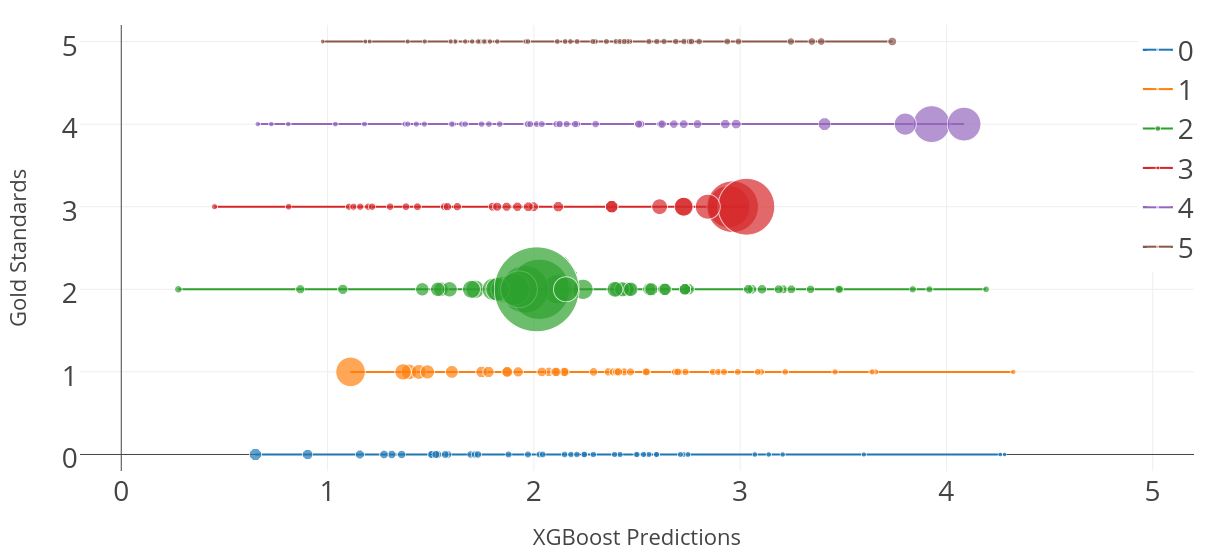
\includegraphics[width=0.92\textwidth]{images/saar-sheff-ans-ans}
    \caption{L1 Error Analysis on the answer-answer domain}
    \label{fig:sts1}
\end{figure}

\begin{figure}[!htb]
    \centering
    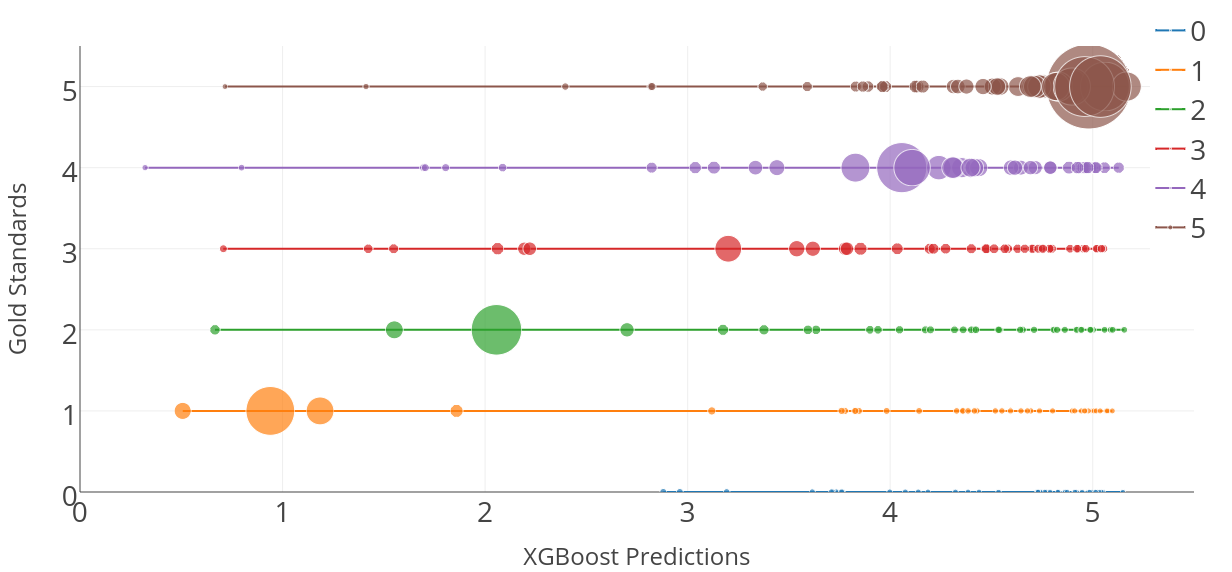
\includegraphics[width=0.92\textwidth]{images/saar-sheff-postediting}
    \caption{L1 Error Analysis on the post-editing domain}
    \label{fig:sts2}
\end{figure}

As we see from Figure \ref{fig:sts1}, the centroids of the bubbles represents our model's best predictions. Our predictions for texts that are annotated at 1 to 4 similarity scores are reasonably close to the gold standards but the model performs poorly for texts annotated with the 0 and 5 similarity scores. 

Looking at the texts that are rated 0, we see that there are cases where the $n$-grams within these texts are lexically / syntactically similar but the meaning of the texts are disparate. For example, this pair of text snippets, \emph{`You don't have to know'} and \emph{`You don't have equipments/facilities'} are rated 0 in the gold standards but from a machine translation perspective, a translator would have to do little work to change \emph{`to know'} to \emph{`equipments/facilities'}. 

Because of this, machine translation metrics would rate the texts as being similar and even suitable for post-editing. However, the STS task focuses only on the meaning of the text which corresponds more to the adequacy aspect of the machine translation metrics. Semantic adequacy is often overlooked in machine translation because our mass reliance on BLEU scores to measure the goodness of translation with little considerations for penalizing semantic divergence between the translation and its reference.

On the other end of the spectrum, machine translation metrics remain skeptical when text snippets are annotated with a score of 5 for being semantically analogous but syntactically the texts are expressed in a different form. For example, given the text snippets, \emph{`There's not a lot you can do about that'} and \emph{`I'm afraid there's not really a lot you can do'}, most machine translation metrics will not allocate full similarity scores due to the difference in lexical and stylistic ways in which the sentences are expressed. 

Machine translation metrics' failure to capture similarity score extremes is evident in Figure \ref{fig:sts1} where there are no 0 and 5.0 predictions. 

Naturally the XGBoost predictions based on the MT evaluation metric features fit the postediting domain. Figure \ref{fig:sts2} shows that the centroids in the L1 Figure for the postediting domain is more centered than in the answer-answer domain.

\subsection{Summary}

In this section, we pursue a combination machine translation evaluation metric {\tt Stasis} to evaluate the grammaticality and semantic adequacy between pairs of sentences. We combined existing machine translation evaluation metrics (that are good in determining fluency) and used linguistically motivated monolingual word alignments and neural embeddings to add the semantic dimension to our new metric.

\newpage
\section{The Awkward Disparity between BLEU / RIBES Scores and
Human Judgments}

Automatic evaluation of machine translation (MT) quality is essential in developing high quality MT systems. 
The relatively consistent correlation of higher BLEU scores \citep{papineni2002bleu} and better human judgements in major machine translation shared tasks has led to the conventional wisdom that translations with significantly higher BLEU scores generally suggests better translation than its lower scoring counterparts \citep{bojar2014findings,WMT15,nakazawa2014overview,cettolo2014report}. 

However, automatic MT evaluation metrics have been criticized for a variety of reasons \citep{babych2004extending,callison2006re}.
\cite{callison2006re} has anecdotally presented possible failures of BLEU by showing examples of translations with the same BLEU score but of different translation quality. Through meta-evaluation\footnote{Meta-evaluation refers to the measurement of the Pearson correlation \emph{R$^2$} between an automatic evaluation metrics and human judgment scores. The meta-evaluation involves the calculation using other correlation measures such as the Spearman's rank correlation $\rho$ \citep{callison2007meta} or the Kendall's Tau $\tau$ \citep{WMT15-metric,graham-baldwin2015}} of BLEU scores and human judgements scores of the 2005 NIST MT Evaluation exercise, they have also showed high correlations of \emph{R$^2$} = 0.87 (for adequacy) and \emph{R$^2$} = 0.74 (for fluency) when an outlier rule-based machine translation system with poor BLEU score and high human score is excluded; when included the correlations drops to 0.14 for adequacy and 0.74 for fluency.


Although Callison-Burch et al. (2006) showed  poor correlation between BLEU and human scores, they had only empirically meta-evaluated a scenario where low BLEU score does not necessary result in a poor human judgement score. 

In this section, we demonstrate a real-world example of machine translation that yielded high automatic evaluation scores but failed to obtain a good score on manual evaluation in an MT shared task submission. In addition to the BLEU metric, we also evaluated our experiments results using the RIBES metric which has previously shown to have better correlations with human judgements due to its sensitivity to reordering \citep{isozaki2010automatic}. 

\subsection{BLEU}

Papineni et al. (2002) originally define BLEU \ngram{} precision \emph{p$_n$} by summing the \ngram{} matches for every hypothesis sentence $S$ in the test corpus $C$:

\begin{equation}\label{eq:bleu-precision}
{ p }_{ n }=\frac { \sum _{ S\in C }^{  }{ \sum _{ ngram\in S }^{  }{ { Count }_{ matched } } (ngram) }  }{ \sum _{ S\in C }^{  }{ \sum _{ ngram\in S }^{  }{ { Count } } (ngram) }  }
\end{equation}

BLEU is a precision based metric; to emulate recall, the brevity penalty (BP) is introduced to compensate for the possibility of high precision translations that are too short. The BP is calculated as:

\begin{equation}\label{eq:bleu-brevity}
BP = \begin{cases}
	\quad 1 \quad \qquad \text{if} \quad c \textgreater r \\
	\quad { e }^{ 1 -r/c} \quad \text{if} \quad c \le r
\end{cases}
\end{equation}

where $c$ and $r$ respectively refers to the length of the hypothesis translations and the reference translations.
The resulting system BLEU score is calculated as follows:

\begin{equation}
	\text{BLEU} = \text{BP} \times  \exp(\sum _{ n=1 }^{ N }{ { w }_{ n } \log { { p }_{ n } }  })
\end{equation}

where $n$ refers to the orders of \ngram{} considered for \emph{p$_n$} and \emph{w$_n$} refers to the weights assigned for the \ngram{} precisions; in practice, the weights are uniformly distributed.

A BLEU score can range from 0 to 1 and the closer to 1 indicates that a hypothesis translation is closer to the reference translation\footnote{Alternatively, researchers would choose to scale the BLEU score to a range between 0 to 100 to improve readability of the scores without the decimal prefix.}.

BLEU is used as the \textit{de facto} standard automatic evaluation metric for major machine translation shared tasks. And BLEU continues to show high correlations primarily for \ngram{}-based machine translation systems \citep{WMT15,nakazawa2014overview}.

However, the fallacy of BLEU-human correlations can be easily highlighted with the following example:

\newpage 
\noindent \textbf{Source}: \\
\begin{CJK*}{UTF8}{}\begin{korean}이러한 작용을 발휘하기 위해서는, \underline{각각} 0.005% 이상 함유하는 것이 바람직하다. \end{korean}\end{CJK*}
\\ \\
\noindent \textbf{Hypothesis}:  \\
\begin{CJK*}{UTF8}{min}このような 作用 を 発揮 する ため に は 、 \underline{夫 々} 0.005 % 以上 含有 する こと が 好ましい 。\end{CJK*}
\\ \\
\noindent \textbf{Baseline}:  \\
\begin{CJK*}{UTF8}{min}このような 作用 を 発揮 する ため に は 、 \underline{それぞれ} 0.005 % 以上 含有 する こと が 好ましい 。\end{CJK*}
\\ \\
\noindent \textbf{Reference}: \\
\begin{CJK*}{UTF8}{min}このような 作用 を 発揮 さ せる ため に は 、 \underline{夫 々 } 0.005 % 以上 含有 さ せる こと が 好ましい 。\end{CJK*}
\\ \\
\textbf{Source/Reference English Gloss}: \\
``So as to achieve the reaction, it is preferable that it contains more 0.005\% of \underline{each} [chemical]''
\vspace{5mm}

The unigram, bigram, trigrams and fourgrams (\emph{p$_1$}, \emph{p$_2$}, \emph{p$_3$}, \emph{p$_4$}) precision of the hypothesis translation are 90.0, 78.9, 66.7 and 52.9 respectively. The \emph{p$_n$} score for the hypothesis sentence precision score for the reference is 70.75. When considering the brevity penalty of 0.905, the overall BLEU is 64.03. Comparatively, the \ngram{} precisions for the baseline translations are \emph{p$_1$}=84.2, \emph{p$_2$}=66.7, \emph{p$_3$}=47.1 and \emph{p$_4$}=25.0 and the overall BLEU is 43.29 with a BP of 0.854. In this respect, one would consider the baseline translation inferior to the hypothesis with a \textgreater10 BLEU difference. However, there is only a subtle difference between the hypothesis and the baseline translation (\begin{CJK*}{UTF8}{min}それぞれ  vs 夫 々\end{CJK*}, which both has the same meaning).

	This is an actual example from the 2\textsuperscript{nd} Workshop on Asian Translation (WAT 2015) MT shared task evaluation, and five crowd-sourced evaluators consider the baseline translation a better translation. For this particular example, the human evaluators preferred the natural translation from Korean \begin{CJK*}{UTF8}{}\begin{korean}각각\end{korean}\end{CJK*} \emph{gaggag} to Japanese \begin{CJK*}{UTF8}{min}それぞれ\end{CJK*} \emph{sorezore} instead of the patent document usage of \begin{CJK*}{UTF8}{min}夫々\end{CJK*} \emph{sorezore}, both \begin{CJK*}{UTF8}{min}それぞれ\end{CJK*} and \begin{CJK*}{UTF8}{min}夫々\end{CJK*} can be loosely translated as '\emph{respectively}' or '\emph{(for) each}' in English.

The big difference in BLEU for a single lexical difference in translation is due to the geometric averaged scores for the individual \ngram{} precisions. It assumes the independence of \ngram{} precisions and accentuates the precision disparity by involving the single lexical difference in all possible \ngram{}s that capture the particular position in the sentence. This is clearly indicated by the growing precision difference in the higher order $n$-grams.

\subsection{RIBES}

Another failure of BLEU is the lack of explicit consideration for reordering. Callison-Burch et al. (2006) highlighted that since BLEU only takes reordering into account by rewarding the higher \ngram{} orders, freely permuted unigrams and bigrams matches are able to sustain a high BLEU score with little penalty caused by tri/fourgram mismatches. To overcome reordering, the RIBES score was introduced by adding a rank correlation coefficient\footnote{normalized Kendall $\tau$ of all \ngram{} pairs between the hypothesis and reference translations} prior to unigram matches without the need for higher order \ngram{} matches \citep{isozaki2010automatic}.

To account for word ordering, the RIBES metric first determines the word rank correlation of the word alignments by computing the Kendall's $\tau$ coefficient. Given the reference and a hypothesis translation:

\begin{enumerate}
  \item[]{\textbf{Reference}:  \textit{Alice kisses Bob yesterday}}
  \item[]{\textbf{Hypothesis}: \textit{Bob kisses Alice yesterday}}
\end{enumerate}


The first word `Alice' in the reference shifted to the third word in the hypothesis and the third word `Bob' becomes the first. The second and fourth word remains intact. From the original [0, 1, 2, 3] word order of the reference, we get the word order list [2, 1, 0, 3] in the hypothesis; where 0 = `\textit{Alice}', 1 = `\textit{kisses}', 2 = `\textit{Bob}' and 3 = `\textit{yesterday}'. 

Given the [2, 1, 0, 3] word order list of the hypothesis, we extract all possible pair of words: [(2, 1), (2, 0), (2, 3), (1, 0), (1, 3), (0, 3)]

The number of all pairs of words can be determined as $\Comb{4}{2}$ = 6. Then, we extract the pairs of words with increasing order, i.e. [(2,3), (1,3), (0,3)].

And the Kendall's $\tau$ coefficient for the word order list is compute as such:

\begin{equation}
\tau = 2 \times \frac{ no. \ of \ increasing \ pairs }{ no. \ of \ all \ pairs } -1
\end{equation}

The $\tau$ for the particular hypothesis in the example above is $\tau$ is 2 x 3/6 - 1 = 0.0. The $\tau$ coefficient ranges between [-1, 1].

To ensure that the final RIBES score ranges between 0.0 to 1.0, th e $\tau$ in the above formulation refers to the normalized Kendall $\tau$ computed as such:

\begin{equation}
\tau_{norm} = (\tau + 1)/2
\end{equation}

Simplifying BLEU's n-th order n-grams precision, the RIBES score only considers the unigram precision, $p_{1}$ using the same Equation \eqref{eq:bleu-precision} with n=1. Similarly, the RIBES brevity penalty, $BP$, follows the BLEU formulation in Equation \eqref{eq:bleu-brevity}

The final RIBES computation scales the unigram precision and brevity penalty by the Kendall's $\tau$ coefficient.

\begin{equation}
RIBES = \tau_{norm} *\ \alpha (p_{1}) *\ \beta (BP)
\end{equation}

where, $\alpha$ and $beta$ are hyperparameter used as a prior for the unigram precision and brevity penalty. They are set as $\alpha$=0.25 and $\beta$=0.10 based on the correlation with human evaluation in \citep{isozaki2010automatic}. 

Let us consider another example:
\\[0.9em]
\noindent \textbf{Source}: \\
\begin{CJK*}{UTF8}{}\begin{korean}T용융 (DSC) = 89.9℃ ; T결정화 (DSC) = 72℃ ( 5℃ / 분에서 DSC 로 측정 ) .\end{korean}\end{CJK*}
\\ \\
\noindent \textbf{Hypothesis}:  \\
\begin{CJK*}{UTF8}{min}Tmelt ( DSC ) = 7 2 ℃( 5 ℃/ 分 で DSC 測定 ( DSC ) = 89 . 9 結晶 化 度 ( T ) 。 \end{CJK*}
\\ \\
\noindent \textbf{Baseline}:  \\
\begin{CJK*}{UTF8}{min}T 溶融 ( DSC ) = 8 9 . 9 ℃; T 結晶 化 ( DSC ) = 7 2 ℃( 5 ℃/ 分 で DSC で 測定 ) 。\end{CJK*}
\\ \\
\noindent \textbf{Reference}: \\
\begin{CJK*}{UTF8}{min}Tmelt ( DSC ) = 8 9 . 9 ℃; Tcryst ( DSC ) = 7 2 ℃( 5 ℃/ 分 で DSC を 用い て 測定 ) 。\end{CJK*}
\\ \\
\textbf{Source/Reference English Gloss}: \\
Tmelt (DSC) = 8 9. 9 $^{\circ}$C; Tcryst (DSC) = 7 $^{\circ}$C (measured using DSC at 5 $^{\circ}$C / min)
\vspace{5mm}

The example above shows the marginal effectiveness of RIBES when penalizing wrongly ordered phrases in the hypothesis. The baseline translation accurately translates the meaning of the sentence with a minor partial translation of the technical variables (i.e. \emph{Tmelt} -> \emph{\begin{CJK*}{UTF8}{min}T 溶融 \end{CJK*}} and \begin{CJK*}{UTF8}{}\begin{korean}T결정화\end{korean}\end{CJK*} -> \emph{\begin{CJK*}{UTF8}{min}T 結晶 化 \end{CJK*}}. However, the hypothesis translation made serious adequacy errors when inverting the values of the technical variables but the hypothesis translation was minimally penalized in RIBES and also BLEU.

The RIBES score for the hypothesis and baseline translations are 94.04 and 86.33 respectively whereas their BLEU scores are 53.3 and 58.8. In the WAT 2015 evaluation, five evaluators unanimously voted in favor for the baseline translation. Although the RIBES score presents a wider difference between the hypothesis and baseline translation than BLEU, it is insufficient to account for the arrant error that the hypothesis translation made.

\subsection{Other Shades of BLEU / RIBES}
It is worth noting that there are other automatic MT evaluation metrics that depend on the same precision-based score with primary differences in how the \emph{Count$_{match}$(ngram)} is measured; \cite{Gimenez2007} described other linguistic features that one could match in place of surface \ngrams{}, such as lexicalized syntactic parse features, semantic entities and roles annotations, etc. As such, the modified BLEU-like metrics can present other aspects of syntactic fluency and semantic adequacy complementary to the string-based BLEU.

A different approach to improve upon the BLEU scores is to allow paraphrases or gappy variants and replace the proportion of \emph{Count$_{match}$(ngram) / \emph{Count(ngram)}} by a lexical similarity measure. \cite{banerjee2005meteor} introduced the METEOR metric that allows hypotheses' \ngram{}s to match paraphrases and stems instead of just the surface strings. \cite{lin-rouges} presented the ROUGE-S metrics that uses skip-gram matches. More recently, pre-trained regression models based on semantic textual similarity and neural network-based similarity measures trained on skip-grams are applied to replace the \ngram{} matching \citep{vela-comet,gupta-reval}.

While enriching the surface \ngram{} matching allows the automatic evaluation metric to handle variant translations, it does not resolve the ``prominent crudeness" of BLEU (Callison-Burch, 2006) involving (i) the omission of content-bearing materials not being penalized, and (ii)  the inability to calculate recall despite the brevity penalty.

\subsection{Experimental Setup}

We describe our experiment setup to evaluate Korean to Japanese patent translation using the Japan Patent Office (JPO) Patent Corpus. The JPO Patent Corpus is the official resource provided for the WAT 2015 shared task. The training dataset is made up of 1 million sentences (250k each from the chemistry, electricity, mechanical engineering and physics domains). Two development datasets\footnote{{\tt dev.txt} and {\tt devtest.txt}} and one test set each comprises 2000 sentences with 500 sentences from each of the training domains. The Korean and Japanese texts were tokenized using KoNLPy \citep{park2014konlpy} and MeCab \citep{kudo2004applying} respectively.

We used the phrase-based SMT implemented in the Moses toolkit \cite{koehn2003statistical,koehn2007moses} with the configurations as described in Chapter 2 (Section 2.4).

\subsubsection{A More Vanilla Baseline System}

\begin{table*}[!ht]
\center
    \begin{tabular}{lcc}
    \textbf{Parameters}                   & \textbf{Organizers} & \textbf{Ours}   \\ \hline
    Input document length                  & 40         & 80     \\
    Korean tokenizer                       & MeCab      & KoNLPy  \\
    Japanese tokenizer                     & Juman      & MeCab \\ \hline
	LM \ngram{} order                      & 5          & 5      \\
    Distortion limit                      & 0          & 20      \\
	Quantized \& binarized LM             & no         & yes    \\
    {\tt devtest.txt} in LM                & no         & yes    \\
    Binarized phrase tables                & no         & yes    \\
    MERT Runs               & 1         & 2    \\
    \end{tabular}
\caption{Differences between Organizer's and our Phrase-based SMT system}
\label{table-diff-between-basline-and-ours}
\end{table*}

Human evaluations were conducted as pairwise comparisons between translations from our system and the WAT organizers' phrase-based statistical MT baseline system. Table~\ref{table-diff-between-basline-and-ours} highlights the parameter differences between the organizers and our phrase-based SMT system. 

\subsubsection{Human Evaluation (Pairwise Comparison)}

The human judgment scores for the WAT evaluations were acquired using the Lancers crowdsourcing platform.
Human evaluators were randomly assigned documents from the test set.
They were shown the source document, %its reference translation, %% according to anonymous reviewer
the hypothesis translation and a baseline translation generated by the phrase-based MT system.
Five evaluators were asked to judge each document.

The crowdsourced evaluators were non-experts, thus their judgements were not necessary precise, especially for patent translations. The evaluators were asked to judge whether the hypothesis or the baseline translation was better, or they were tied. The translation that was judged better constituted a \emph{win} and the other a \emph{loss}. For each, the majority vote between the five evaluators for the hypothesis decided whether the hypothesis \emph{won}, \emph{lost} or \emph{tied} the baseline.  The final human judgment score, \emph{HUMAN}, is calculated as follows:
\begin{equation}
	\text{HUMAN} = 100 \times \frac { W-L }{ W+L+T }
\end{equation}

By definition, the \emph{HUMAN} score ranges from $-100$ to $+100$, where higher is better.

\subsection{Results}

Moses' default parameter tuning method, \mert{}, is non-deterministic, and hence it is advisable to tune the phrase-based model more than once (Clark et al. 2011). We repeated the tuning step and submitted the system translations that achieved the higher BLEU score on the development set for manual evaluation.

As a sanity check we also replicated the organizers' baseline system and submitted it for manual evaluation. We expect this system to score close to zero. We submitted a total of three sets of output to the WAT 2015 shared task, two of which underwent manual evaluation.

\begin{table}[!ht]
\center
    \begin{tabular}{lccc}
    \textbf{Systems}           & \textbf{RIBES} & \textbf{BLEU}  & \textbf{HUMAN}  \\ \hline
    Organizers'            	   &  				&   \\
    PBMT baseline         	   & 94.13				& 69.22 	& 0.0      \\ \hline
    Our  replica     		   &				& 				& \    \\
    baseline    			   & 94.29				& 70.23   & \textbf{+3.50}    \\
	Ours (\mert{} 1)              & 95.03				& 84.26 			& -      \\
	Ours (\mert{} 2)              & \textbf{95.15}				& \textbf{85.23} & -17.75 \\

    \end{tabular}
\caption{BLEU and HUMAN scores for WAT 2015}
\label{table-bleu-and-human-scores}
\end{table}

Table~\ref{table-bleu-and-human-scores} presents the BLEU scores achieved by our phrase-based MT system in contrast to the organizers' baseline phrase-based system. The difference in BLEU between the organizers' system and ours may be due to our inclusion of the second development set in building our language model and the inclusion of more training data by allowing a maximum of 80 tokens per document as compared to 40 (see Table~\ref{table-diff-between-basline-and-ours}). 

% Another major difference is the high distortion limit we have set as compared to the organizers' monotonic system, it is possible that the high distortion limit compensates for the long distance word alignments that might have been penalized by the phrasal and reordering probabilities which results in the higher RIBES and BLEU score.\footnote{In our submission {\tt Byte2String} refers to the encoding problem we encountered when tokenizing the Korean text with MeCab causing our system to read Korean bytecode instead of Unicode. But the decoder could still output Unicode since our Japanese data was successfully tokenized using MeCab, we submitted this output under the submission name {\tt Byte2String}; the {\tt Byte2String} submission is not reported in this paper. Later we rectified the encoding problem by using KoNLPy and re-ran the alignment, phrase extraction, MERT and decoding, hence the submission name, {\tt Unicode2String}, i.e. the system reported in Table~\ref{table-bleu-and-human-scores}.}

However, the puzzling fact is that our system being 15 BLEU points better than the organizers' baseline begets a terribly low human judgement score. We discuss this next.

\subsection{Segment Level Meta-Evaluation}

\begin{figure}[!htb]
    \centering
    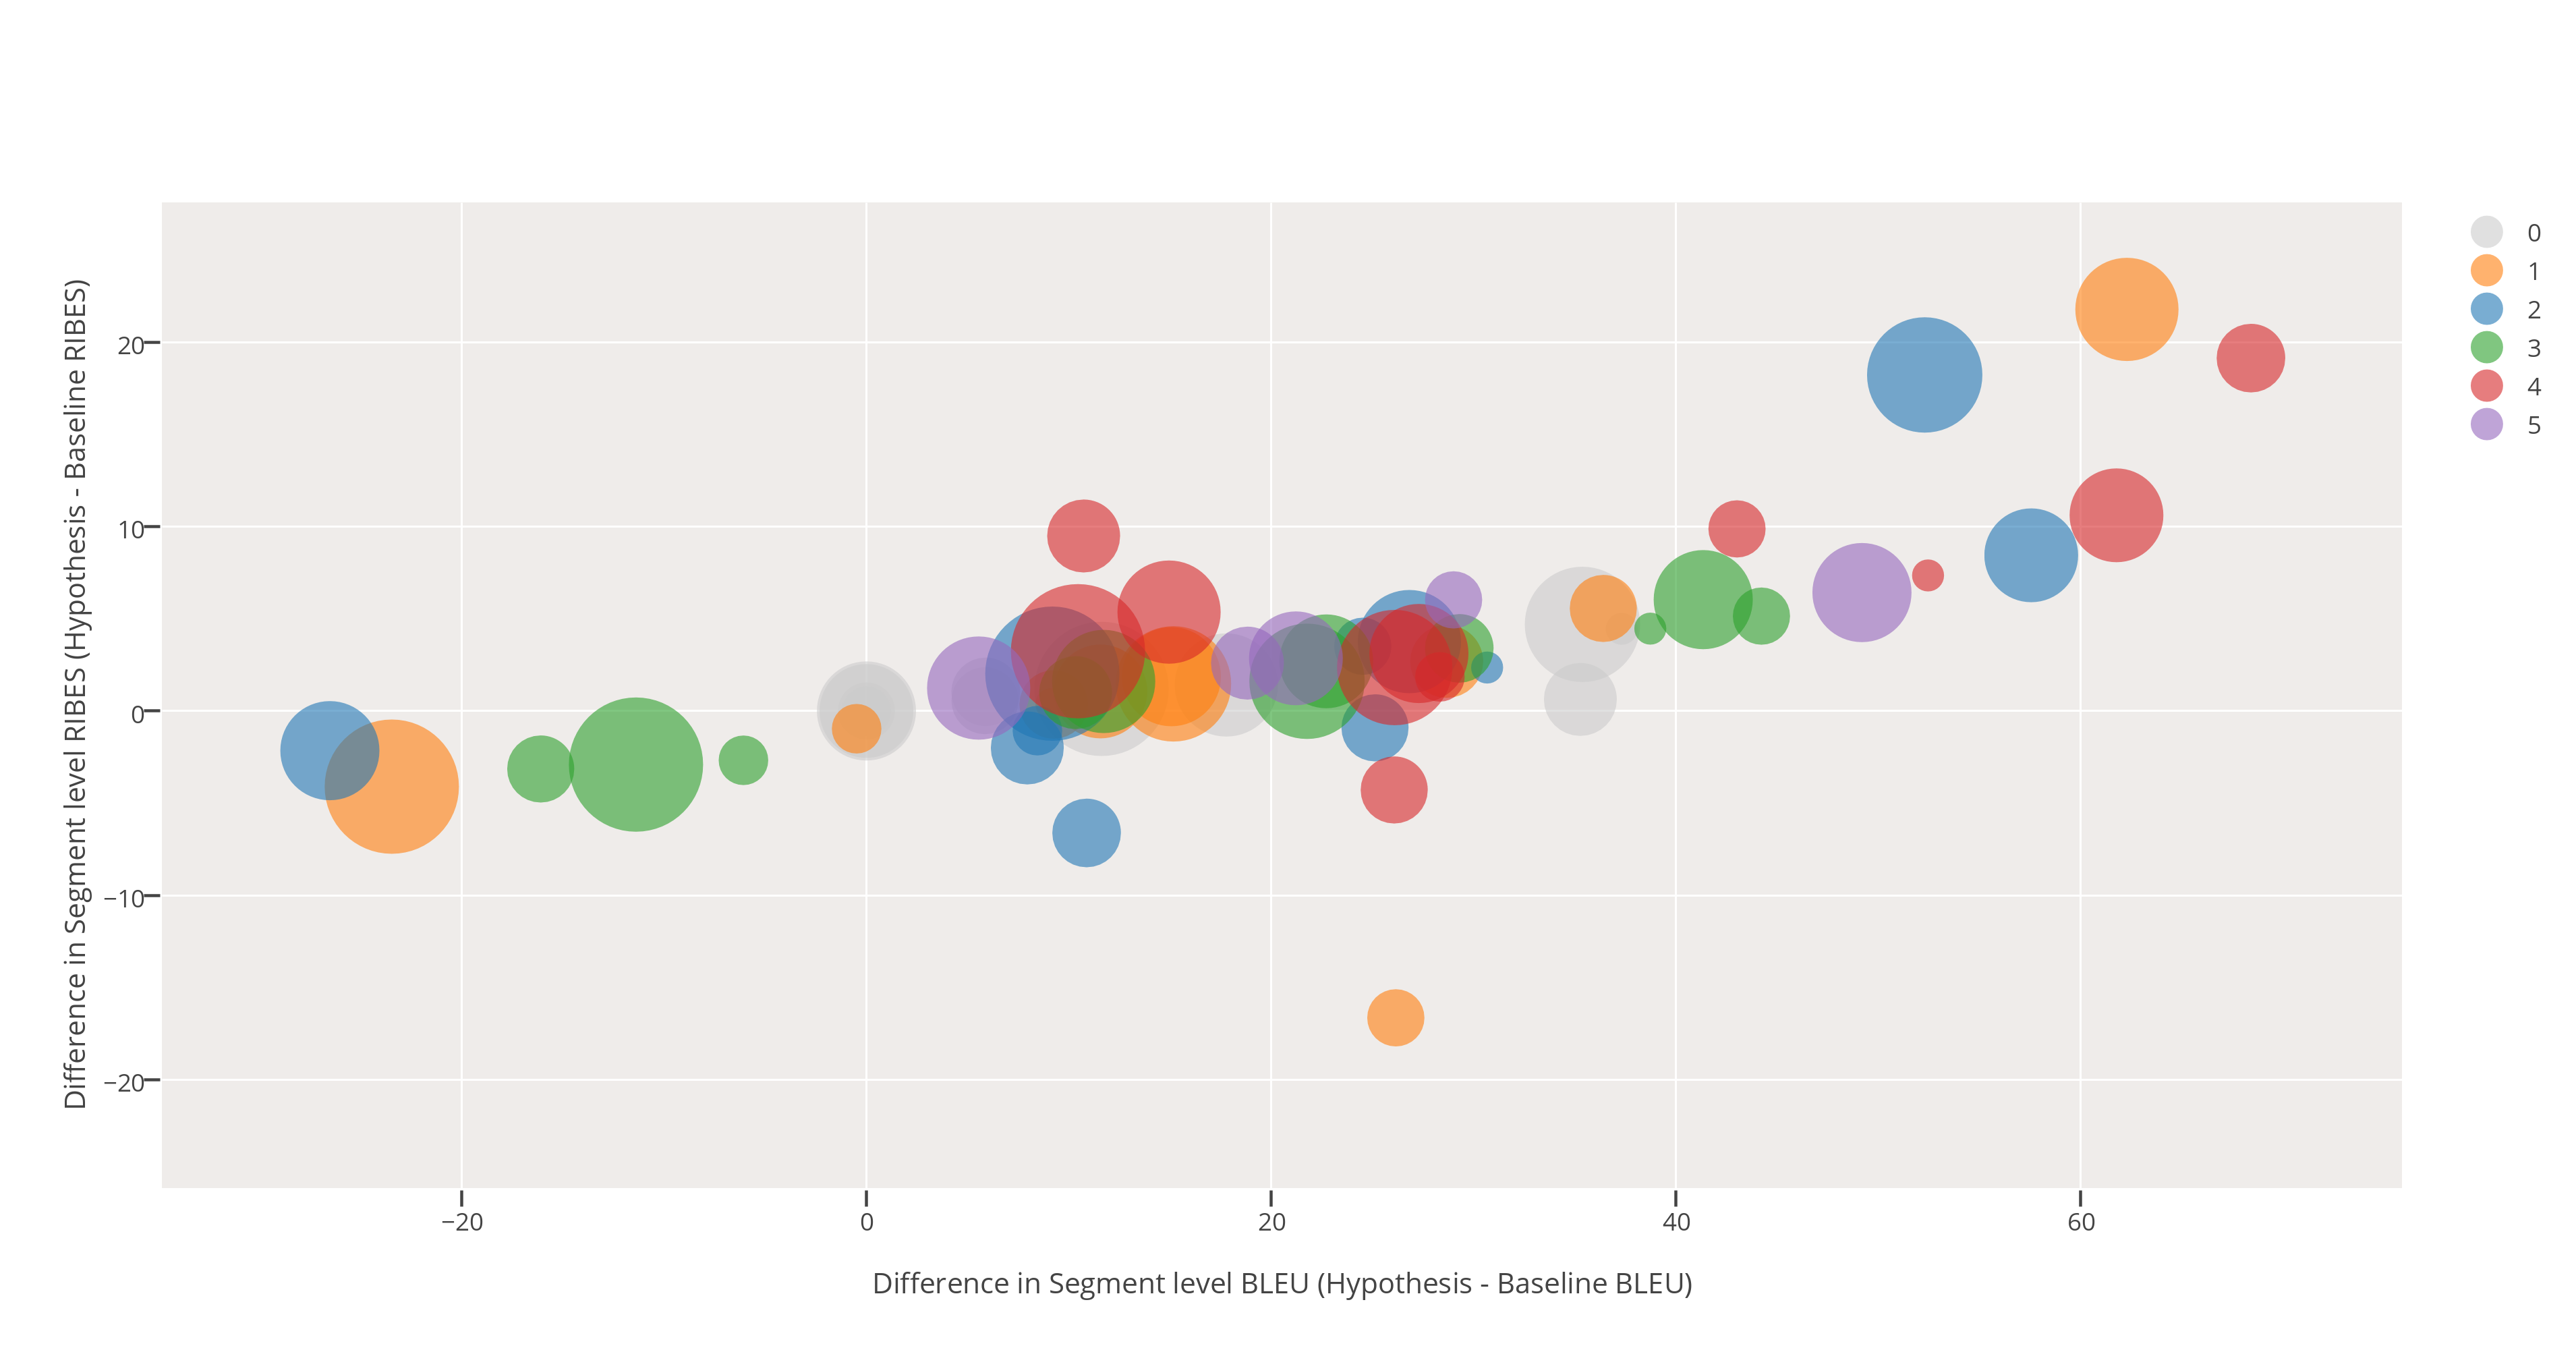
\includegraphics[width=0.8\textwidth]{diff-bleu-ribes-positive}
    \caption{Correlation between BLEU, RIBES differences and \emph{\underline{Positive}} HUMAN Judgements (HUMAN Scores of 0, +1, +2, +3, +4 and +5 represented by the colored bubbles: \emph{grey, orange, blue, green, red and purple}; larger area means more segments with the respective HUMAN Scores)}
\label{fig-cor-pos}
\end{figure}

\begin{figure}[!htb]
    \centering
    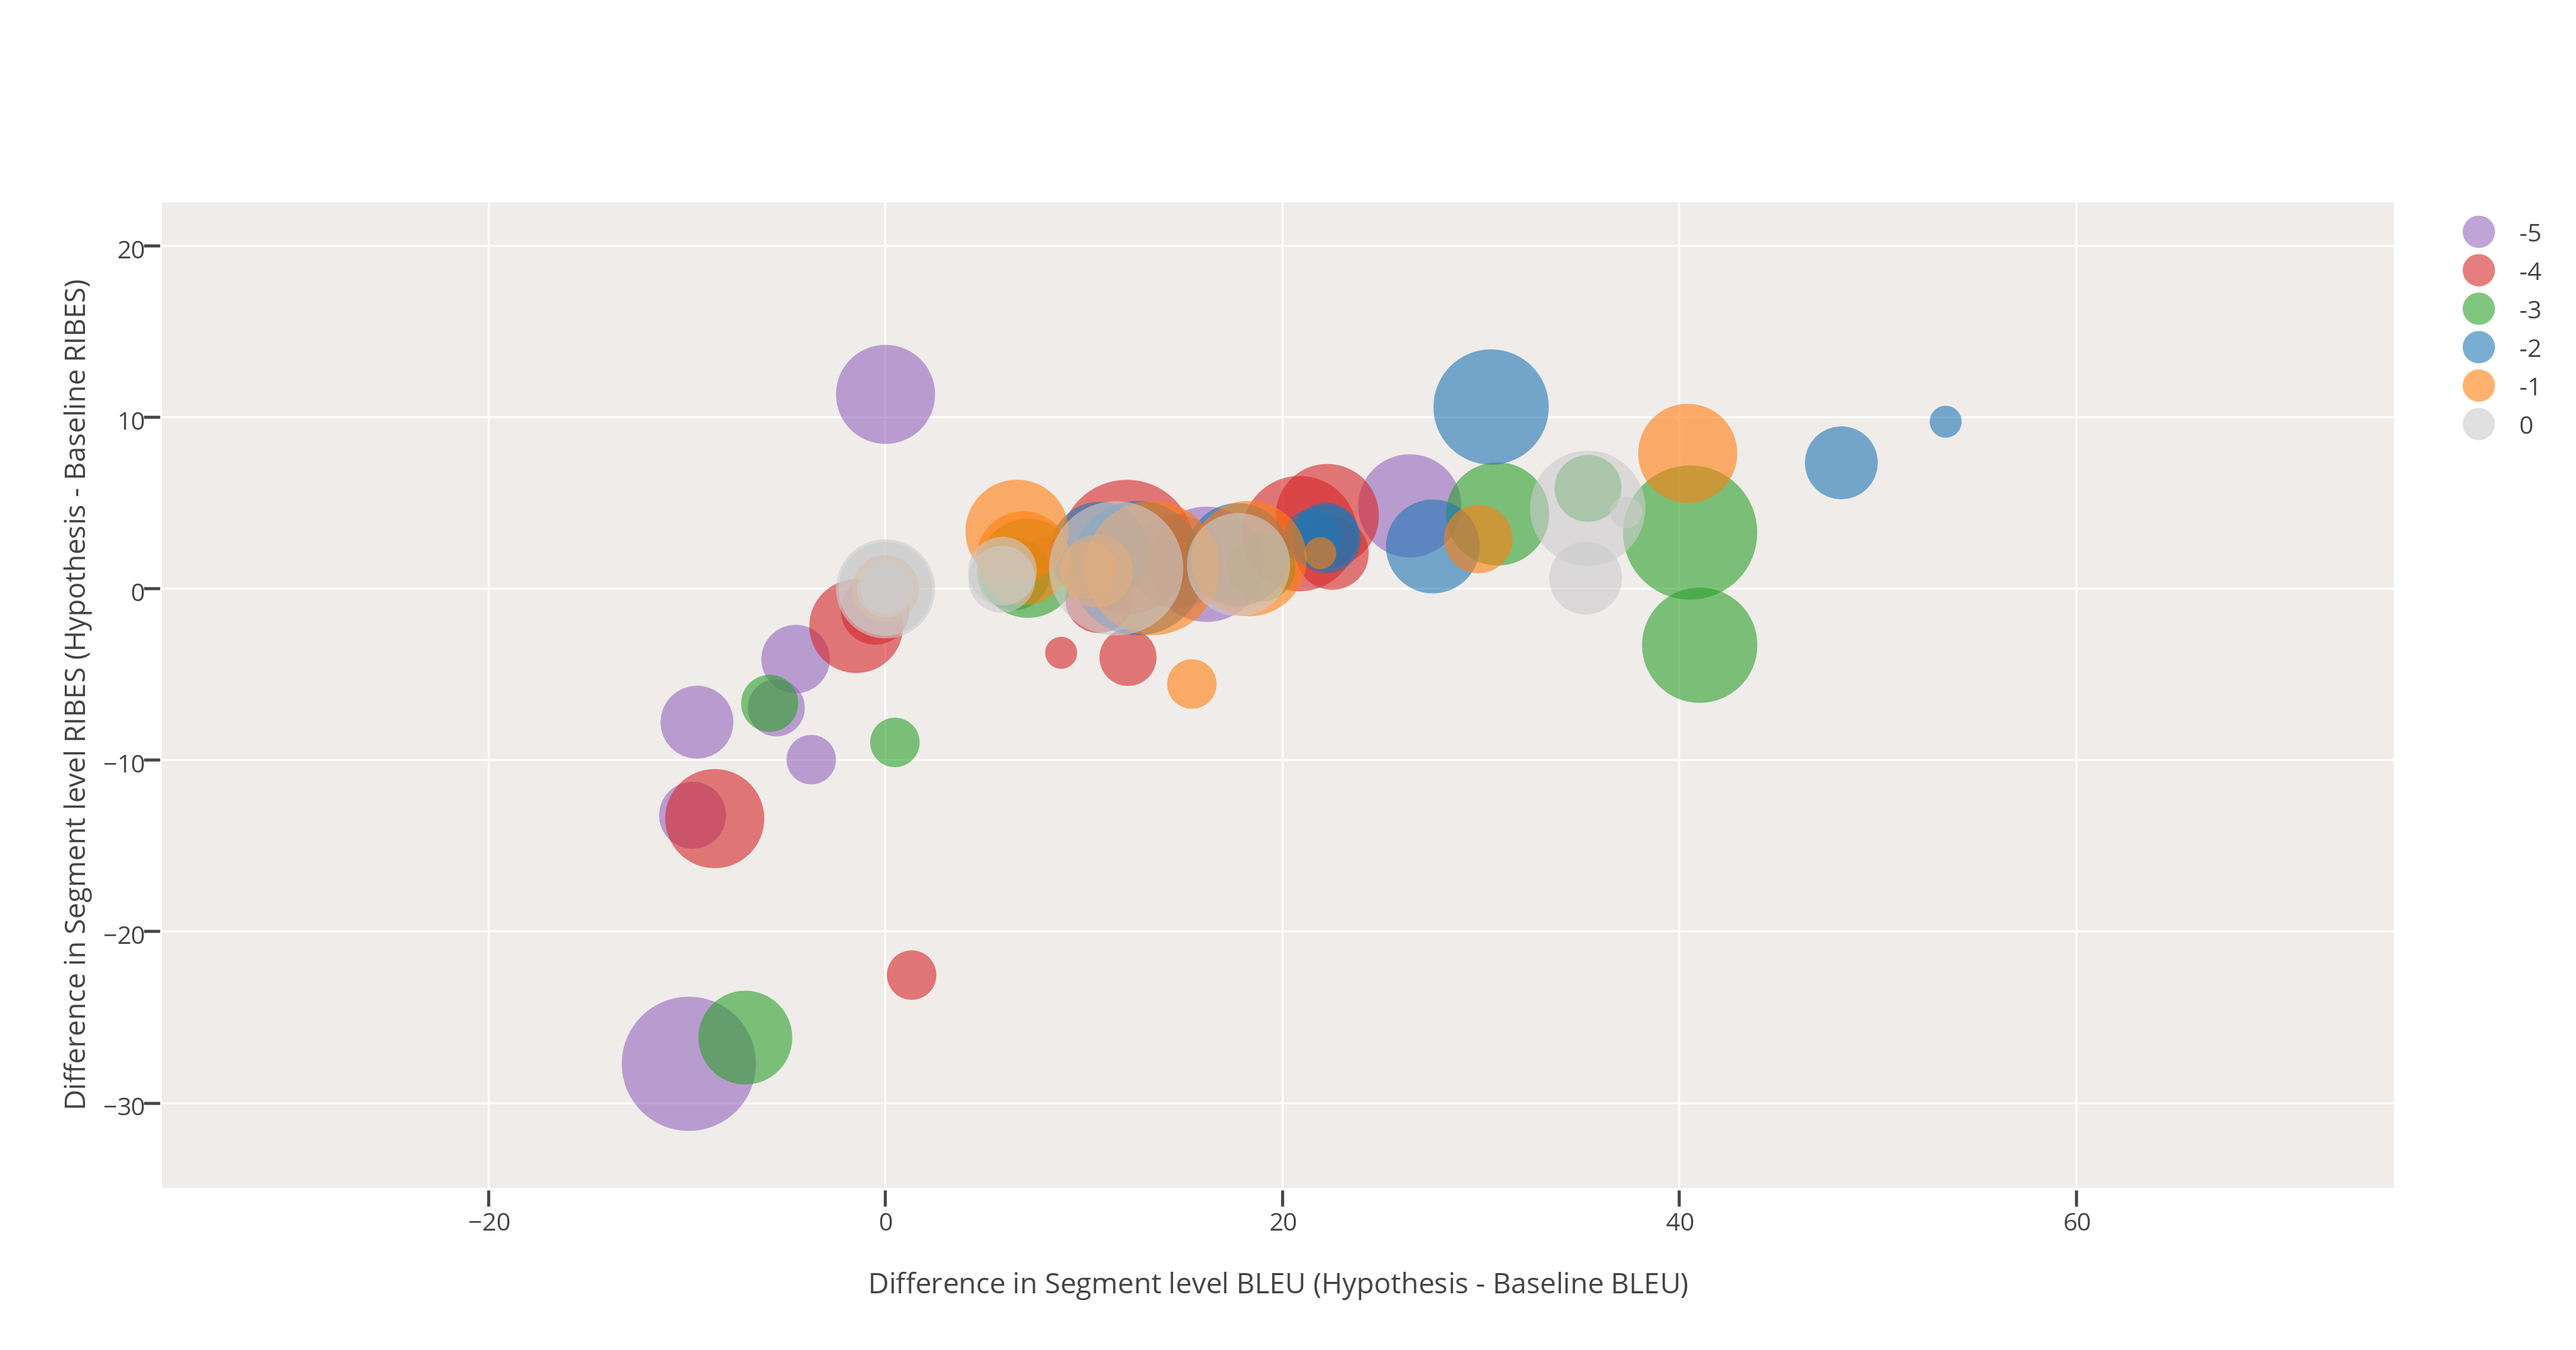
\includegraphics[width=0.8\textwidth]{diff-bleu-ribes-negative}
    \caption{Correlation between BLEU, RIBES differences and \underline{\emph{Negative}} HUMAN Judgements (HUMAN Scores of 0, -1, -2, -3, -4 and -5 represented by the colored bubbles: \emph{grey, orange, blue, green, red and purple}; larger area means more segments with the respective HUMAN Scores)}
\label{fig-cor-neg}
\end{figure}

We perform a segment level meta-evaluation by calculating the BLEU and RIBES score difference for each hypothesis-baseline translation. Figures~\ref{fig-cor-pos} and \ref{fig-cor-neg} show the correlations of the BLEU and RIBES score difference against the positive and negative human judgements score for every sentence.

Figure~\ref{fig-cor-pos} presents the considerable incongruity between our system's high BLEU improvements (>+60 BLEU) being rated marginally better than the baseline translation, indicated by the orange and blue bubbles on the top right corner. There were even translations from our system with >+40 BLEU improvements that tied with the organizer's baseline translations, indicated by the grey bubbles at around the +40 BLEU and +5 RIBES region. Except for a portion of segments that scored worse than the baseline system (lower right part of the graph where BLEU and RIBES falls below 0), the overall trend in Figure~\ref{fig-cor-pos} presents the conventional wisdom that the BLEU improvements from our systems reflects positive human judgement scores.

However, Figure~\ref{fig-cor-neg} presents the awkward disparity where many segments with BLEU improvements were rated strongly as poorer translations when compared against the baseline. Also, many segments with high BLEU improvements were tied with the baseline translations, indicated by the grey bubbles across the positive BLEU scores.

As shown in the examples in Section 2, a number of prominent factors contribute to this disparity between high BLEU / RIBES improvements and low HUMAN judgement scores:
\begin{itemize}
	\item Minor lexical differences causing a huge difference in \ngram{} precision
	\item Crowd-sourced \textit{vs}.\ expert preferences on terminology, especially for patents
	\item Minor MT evaluation metric differences not reflecting major translation inadequacy
\end{itemize}

Each of these failures contributes to an increased amount of disparity between the automatic translation metric improvements and human judgement scores.

\subsection{Summary}

In this section, we have demonstrated a real-world case where high BLEU and RIBES scores do not correlate with better human judgement. We presented several factors that might contribute to the poor correlation, and also performed a segment level meta-evaluation to identify segments where our system's high BLEU\,/\,RIBES improvements were deemed substantially worse than the baseline translations. 
We hope our results and analysis will lead to improvements in automatic translation evaluation metrics. 

\newpage
\section{Summary}

Taking a short detour from terminology and ontology, Section 6.1 and 6.2 in this chapter presented our first attempt in mitigating the inadequacy of current state-of-art machine translation evaluation metrics and propose a semantically motivated metric by casting the machine translation task as a semantic textual similarity task. Then we explored the discrepancy between automatic machine translation evaluation metrics against the human judgments of the quality of the translated text and we found an awkward disparity between them. We hope that the findings in this chapter can help in future studies in the measurement of machine translation quality and eventually improve machine translation in turn. 

%\section{Cleaning Data for the Win}
%\subsection{Gale-Church Filter} % If I've time, the symmetrized version.

%\section{Tuning Systems}
%\subsection{with Harmonic MERT-MIRA Weights}
%\subsection{with Linear Regression PRO}
%\subsection{with Tree-LSTM}

%\subsection{COMET Evaluation Metric}
%\subsection{BFF Quality Estimation}

%%%%%%%%%%%%%%%%%%%%%%%%%%%%%%%%%%%%%%%%%%%%%%%%%%%%%%%%%%%%%%%%%%%%
% Ontology Induction with Neural Nets
%%%%%%%%%%%%%%%%%%%%%%%%%%%%%%%%%%%%%%%%%%%%%%%%%%%%%%%%%%%%%%%%%%%%

\chapter{Ontology Induction using Neural Vector Space}
\label{chap:ontoinduce}

Semantic ontologies provide structured world knowledge to Artificial Intelligence (AI) and Natural Language Processing (NLP) systems. Traditional broad-coverage taxonomies such as CYC \citep{lenat1995cyc}, SUMO \citep{Pease2002Suggested,Miller1995}, YAGO \citep{Suchanek2007} and Freebase \citep{Bollacker2008} have been manually created or curated with much effort and yet they suffer from coverage sparsity. This motivated the move towards unsupervised approaches to extract structured relational knowledge from texts \citep{lin2001discovery,snow2006semantic,velardi2013ontolearn}.

With the rapid technological evolution, it is more feasible to automatically construct a domain-specific taxonomy that caters to sector or company specific terminology \citep{lefever:2015:SemEval}. This motivated the move towards unsupervised approaches to taxonomy extraction \citep{berland1999finding,lin2001discovery,snow2006semantic} and specifically focused towards particular domains \citep{velardi2013ontolearn,bordea-EtAl:2015:SemEval}. 

Previous work in taxonomy extraction focused on rule-based, clustering and graph-based approaches. The hierarchical structure of domain concepts is made up of hypo-hypernymy relations between terms. Different approaches have been proposed to induce these relations automatically ranging from pattern/rule-based approaches \citep{hearst1992,girju2003automatic,kozareva2008,ceesay-juanhou:2015:SemEval} to clustering and frequency based approaches \citep{lin1998automatic,Caraballo2001,pantelravi2004,grefenstette:2015:SemEval}, classification approaches \citep{snow2004learning,ritter2009anyway,espinosaanke-saggion-ronzano:2015:SemEval} and graph-based approaches \citep{kozareva2010semi,navigliVF11,fountain2012taxonomy,Tuan2014,cleuziou-EtAl:2015:SemEval} (See Chapter 2, Section 2.5.3). 

More recently, there is a resurgence of vector space or distributional approaches \citep{van2005automatic,lenci2012identifying,santus2014} primarily because of the renaissance of deep learning and network networks. Semantic knowledge can be thought of as a vector space where each word is presented by a point and the proximity between words in this space quantifies their semantic association. The vector space is usually constructed from the distribution of words across context such that similar meanings tend to be found close to each other within the vector space \citep{Mitchell:Lapata:2010}. 

With the present advancement in neural nets and word embeddings \citep{mikolov2013distributed,pennington2014glove,levy2014linguistic,shazeer2016swivel}, neural space models are gaining popularity in taxonomy induction and relation extraction tasks \citep{saxe2013,fu2014semhierarchies,tan-gupta-vangenabith:2015:SemEval}.

Fu et al. (2014) proposed a vector space approach to hypernym identification using word embeddings that trains a projection matrix that converts a hyponym vector to its hypernym. However, their approach requires an existing hypernym-hyponym pairs for training before discovering new pairs.

Instead of learning a supervised transition matrix $\Phi$, we capitalize on the fact that hypernym-hyponym pairs often occur in a sentence with an ‘is a’ phrase, e.g. “The goldfish (Carassius auratus auratus) is a freshwater fish”.\footnote{\url{http://en.wikipedia.org/wiki/Goldfish}}

We propose a simpler unsupervised approach where we learn a vector for the phrase ``\emph{is-a}". We single-tokenize the adjacent ``is" and ``a" tokens and learn the word embeddings with \emph{is-a} forming part of the vocabulary in the input matrix. 

\section{Inducing a Hypernym with \emph{is-a} Vector}

Effectively, we hypothesize that $\Phi$ can be replaced by the ``\emph{is-a}" vector. To achieve the piecewise projection effects of $\Phi$, we trained a different deep neural net model for each Taxonomy Extraction Evaluation (TaxEval) domain \citep{task17semeval2015} and assume that the ``\emph{is-a}" scales automatically across domains. For instance, the multiplication  of the \emph{v}\texttt{(tiramisu)} and the \emph{v}\texttt{(is-a$_{food}$)} vectors yields a proxy vector and we consider the top ten word vectors that are most similar to this proxy vector as the possible hypernyms, i.e. \emph{v}\texttt{(tiramisu)}$\times$\emph{v}\texttt{(is-a$_{food}$)} $\approx$ \emph{v}\texttt{(cake)}.

There is little or no previous work that manipulates non-content word vectors in vector space models for natural language processing. Often, non-content words\footnote{Words that are not noun (entities/arguments), verbs (predicates), adjectives or adverbs (adjuncts).} were implicitly incorporated into the vector space models by means of syntactic frames or syntactic parses \citep{Sarmento2009}.

Our main contribution for ontological induction using vector space models are primarily (i) the use of non-content word vectors and (ii) simplifying a previously complex process of learning a hyper-hyponym transition matrix\footnote{Parts of the research reported in this chapter has been published in \cite{tan-gupta-vangenabith:2015:SemEval}}.

\subsection{Experimental Setup}

Similar to \cite{fountain2012taxonomy}, the SemEval-2015 Taxonomy Extraction Evaluation (TaxEval) task addresses taxonomy learning without the term discovery step, i.e. the terms for which to create the taxonomy are given \citep{task17semeval2015}. The focus is on creating the hypernym-hyponym relations. We will be using this dataset to evaluate our hypernym induction system using the \textit{`is-a'} vector.

In the TaxEval task, ontologies are evaluated through comparison with gold standard taxonomies. There is no training corpus provided by the organisers of the task and the participating systems are to generate hyper-hyponyms pairs using a list of terms from four different domains, viz. chemicals, equipment, food and science. 

The gold standards used in evaluation are the \emph{ChEBI ontology} for the chemical domain \citep{degtyarenko2008chebi}, the \emph{Material Handling Equipment taxonomy}\footnote{http://www.ise.ncsu.edu/kay/mhetax/index.htm} for the equipment domain, the \emph{Google product taxonomy}\footnote{http://www.google.com/basepages/producttype/taxonomy.en-US.txt} for the food domain and the\emph{ Taxonomy of Fields and their Different Sub-fields}\footnote{http://sites.nationalacademies.org/PGA/Resdoc/PGA\_044522} for the science domain. In addition, all four domains are also evaluated against the sub-hierarchies from the WordNet ontology that subsumes the Suggested Upper Merged Ontology \citep{PeaseEtAl2002sumo}.

There is no specified training corpus released for the SemEval-2015 TaxEval task. To produce a domain specific corpus for each of the given domains in the task, we used the Wikipedia dump and preprocessed it using WikiExtractor\footnote{We use the same Wikipedia dump to text extraction process from the SeedLing - Human Language Project \citep{emerson2014}.} and then extracted documents that contain the terms for each domain individually.

We trained a skip-gram model phrasal word2vec neural net \citep{mikolov2013efficient} using gensim \citep{rehureklrec}. The neural nets were trained for 100 epochs with a window size of 5 for all words in the corpus.

\subsection{Evaluation Metrics}

For the TaxEval task, the multi-faceted evaluation scheme presented in Navigli (2013) was adopted to compare the overall structure of the taxonomy against a gold standard, with an approach used for comparing hierarchical clusters. The multi-faceted evaluation scheme evaluates (i) the structural measures of the induced taxonomy (left columns of Table 6.1), (ii) the comparison against gold standard taxonomy (right columns of Table 6.1 and leftmost column of Table 6.2) and (iii) manual evaluation of novel edges precision (last row of Table 6.2). 

Regarding the two types of automatic evaluation measures, the structural measures provide a gauge of the system's coverage and the ontology structural integrity, i.e. ``tree-likeness" of the ontology produced by the hypernym-hyponym pairs, and the comparison against the gold standards gives an objective measure of the ``human-likeness" of the system in producing a taxonomy that is similar to the manually-crafted taxonomy.

\section{Results}


\begin{table}[H]
\small
\centering
    \begin{tabular}{l|cccc|ccccc}
                 & \textbf{$\vert$V$\vert$}   & \textbf{$\vert$E$\vert$}   & \textbf{\#c.c} & \textbf{cycles} & \textbf{\#VC} & \textbf{\%VC} & \textbf{\#EC} & \textbf{\%EC} & \textbf{:NE} \\ \hline
    \textbf{Chemical}     & 13785 & 30392 & 302    & YES    & 13784                 & \textbf{0.7838}          & 2427               & 0.0977        & 1.1268               \\
    \textbf{Equipment}    & 337   & 548   & 28     & YES    & 336                   & 0.549           & 227                & 0.3691        & 0.5219               \\
    \textbf{Food}         & 1118  & 2692  & 23     & YES    & 948                   & 0.6092          & 428                & 0.2696        & 1.4265               \\
    \textbf{Science}      & 355   & 952   & 14     & YES    & 354                   & 0.7831          & 173                & \textbf{0.3720}         & 1.6752               \\ \hline
   \textbf{WN Chemical}  & 1173  & 3107  & 31     & YES    & 1172                  & \textbf{0.8675}          & 532                & \textbf{0.3835}       & 1.8566               \\
    \textbf{WN Equipmen}t & 354   & 547   & 43     & YES    & 353                   & 0.7431          & 149                & 0.3072        & 0.8206               \\
    \textbf{WN Food }     & 1200  & 3465  & 23     & YES    & 1199                  & 0.8068          & 549                & 0.3581        & 1.9021               \\
   \textbf{WN Science }  & 307   & 892   & 8      & YES    & 306                   & 0.7132          & 156                & 0.3537        & 1.6689               \\
    \end{tabular}
    \caption{Structural Measures and Comparison against Gold Standards for {\tt USAAR-WLV}. The labels of the columns refer to 
no. of distinct vertices and edges in induced taxonomy (\textbf{$\vert$V$\vert$} and \textbf{$\vert$E$\vert$}), 
no. of connected components (\textbf{\#c.c}), whether the taxonomy is a Directed Acyclic Graph (\textbf{cycles}),
vertex and edge coverage, i.e. proportion of gold  standard vertices and edges covered by system (\textbf{\%VC} and \textbf{\%EC}), 
no. of vertices and edges in common with gold standard (\textbf{\#VC} and \textbf{\#EC}) and ratio of novel edges (\textbf{:NE}).}
\end{table}

\begin{table}[H]
\small
\centering
    \begin{tabular}{l|ccccc|c}
             & \textbf{INRIASAC} & \textbf{LT3}    & \textbf{NTNU}   & \textbf{QASSIT} & \textbf{TALN-UPF} & \textbf{USAAR} \\ \hline
    Avg. F\&M & 0.3270 & \textbf{0.4130} & 0.0580 & 0.3880 & 0.2630 & 0.0770 \\
    Avg. Precision   & 0.1721   & \textbf{0.3612} & 0.1754 & 0.1563 & 0.0720    & 0.2014    \\
    Avg. Recall   & 0.4279   & \textbf{0.6307} & 0.2756 & 0.1588 & 0.1165   & 0.3139    \\
    Avg. F-Score   & 0.2427   & \textbf{0.3886} & 0.2075 & 0.1575 & 0.0798   & 0.2377    \\
   Avg. Precision of NE & 0.4800    & \textbf{0.5960}  & 0.3530  & 0.2470  & 0.1020    & 0.4200     \\
    \end{tabular}
    \caption{Averaged F\&M Measure, Precision, Recall, F-score for All Systems Outputs when Compared to Gold Standard and Manually Evaluated Average Precision of Novel Edges.}
\end{table}

Table 6.2 presents the evaluation scores for our system (USAAR) in the TaxEval task, the \%VC and \%EC scores summarize the performance of the system in replicating the gold standard taxonomies. 

In terms of vertex coverage, our system performs best in the chemical and WordNet chemical domain. Regarding edge coverage, our system achieves highest coverage for the science domain and WordNet chemical domain. Having high edge and vertex coverage significantly lowers false positive rate when evaluating hypernym-hyponyms pairs with precision, recall and F-score. 

We also note that the wikipedia corpus extracted that we used to induce the vectors lacks coverage for the food domain. In the other domains, we discovered all terms in the wikipedia corpus plus the domains' root hypernym (i.e. \textbf{$\vert$V$\vert$} = \textbf{\#VC} + 1).

Table 6.2 presents the comparative results between the participating teams in the TaxEval task averaged over all domains. We performed reasonably well as compared to the other systems in all measures. While our system's Fowlkes and Mallows measure (F\&M) is low, it is only representative of the clusters we have induced as compared to the gold standard. To improve our F\&M measure, we could reduce the number of redundant novel edges by pruning our system outputs and achieve comparable results to the other teams given our relatively precision of novel edges.

\section{Hyponym Endocentricity}

Early research in theoretical linguistics discussed the idea of \emph{endocentric} vs. \emph{exocentric} constructions \citep{brugmann1886vergleichende,aleksandrov1886sprachliches,brockelmann1908grundriss,bloomfield1983introduction}. 

A grammatical construction is \emph{endocentric} when it fulfils the same linguistic function as one of its parts. For instance, the word \emph{goldfish} is an endocentric compound noun that shares the syntactic noun properties of \emph{fish} and semantically the compound denotes a type of \emph{fish}. 

Conversely, when a grammatical construction made up of two or more parts is not \emph{endocentric}, the construction would be exocentric such that no one part of the construction contains the main meaning of the word. Intuitively, we can perceive that there are many endocentric hyponyms in a taxonomy where part of the term conveys its main meaning and usually that part of term would be its hypernym.

While experimenting with ways to weight a term for information retrieval, \cite{jones1979experiments} observed that compound nouns follow the head-modifier principle where the meaning of the term can be conveyed by part(s) of the compound. In the first TExeval task in SemEval-2015, both \cite{lefever:2015:SemEval} and \cite{tan-gupta-vangenabith:2015:SemEval}\footnote{https://github.com/alvations/USAAR-SemEval-2015/tree/master/task17-USAAR-WLV} independently developed string-based systems that exploit the endocentric nature of hyponyms. 

%The endo/exocentricity feature of any lexical term assumes that the term can be split up into two or more parts. For example, \emph{fish} is a single noun that cannot be split up thus it cannot be endo- or exocentric. 

In this section, we seek to answer the question of exactly \textbf{\emph{``how many of hyponyms within a taxonomy are endocentric?"}}. Additionally, we exploit the endocentric nature of the hyponyms to extend the taxonomy by trawling Wikipedia \emph{List of Lists of Lists}\footnote{https://en.wikipedia.org/wiki/List\_of\_lists\_of\_lists}. Often these lists of terms are found in Wikipedia marked up tables or in bullet forms.

\subsection{Identifying Endocentric Parts}

The main implementation of the rule-based identifier\footnote{Our open-source implementation can be found at https://github.com/alvations/Endrocentricity} checks \textbf{\emph{if a term T1 is a substring of T2} and if so, \emph{assign T1 as a hypernym of T2}}. Examples of hypo-hypernym pairs captured by this rule includes are (\emph{linguistics, psycholinguistics}), (\emph{beef, kobe beef}), (\emph{sauce, sauce gribiche}). 

Our implementation is a little simpler than the three part morpho-syntactic analyzer component of the multi-modular taxonomy constructor in \cite{lefever:2015:SemEval}. She implemented rules for three different syntactic constructions where they check for suffix and treat single-word terms and multi-word terms differently while our implementation is agnostic to the single and multi-word distinction. 

In addition to first, \emph{\textbf{if a term contains the ``of" preposition, we swap the assignment and check that T2 starts with T1 then assign T2 as a hypernym of T1}}. Examples of hypo-hypernym pairs captured by this swap rule are (\emph{elixir of life, elixir}), (\emph{sociology of education, sociology}). 

To improve the precision of the identifier, we set a threshold of a minimum character length of three when identifying a term as a hypernym. 

\section{Extending Taxonomy with Wikipedia List of Lists of Lists}

The Wikipedia List of Lists of Lists (LOLOL) is a crowd-sourced list of lists of terms that belong to their respective categories.  We adapted the a customized crawler\footnote{It was built for crawling translations and diachronic texts in previous SemEval tasks} \citep{tan-EtAl:2014:SemEval,tan-ordan:2015:SemEval} to crawl for tables or bullet points in Wikipedia the subpages of the LOLOL for the food domain. We started the crawl from these seed pages under the bullet point of \url{ https://en.wikipedia.org/wiki/List\_of\_lists\_of\_lists\#Food\_and\_drink}.

When the crawler lands on each List of List (LOL) page, it will \emph{\textbf{treat the URL suffix as the hypernym}} and \emph{\textbf{find words in the bullet points or tables that contains endocentric hyponyms}}. 

If an endocentric hyponym exists, it will extract either extract (i) all the bolded terms if the LOL page is bulletined or (ii) all terms in the first column if the LOL page is in table form. The choice of the first column is based on the fact that often LOL tables are bi-column, one containing the terms and the other the gloss or/and description of the term.

\subsection{Limitations of LOLOL Trawler}

However, there are a couple issues with this \emph{\textbf{trawling}} (\emph{crawl+clean}) approach to extend the taxonomy.
%\footnote{Due to the non-server friendly implementation of our trawler, the source is not openly released. It will try to bypass {\tt robot.txt}}. 

\textbf{LOL Pages are Not Standardized}: The way the crawler cleans the bullets or tables on each LOL page is not standardized because there is not constraint put on the format of the Wikipedia's LOL page, our crawler only managed to crawl and clean less than 10 LOL pages when extracting the new terms for the food domain. 

\textbf{LOL Pages are Inceptive}: The depth of how nested the LOLs are is undefined. Our crawler can start with a {\tt List\_of\_foods} page and it leads to the {\tt List\_of\_breads} page and then the {\tt List\_of\_American\_breads} page and it continues. For sanity, we had to break our trawler at the second page depth and return to the main LOLOL page to move on to the next LOL that we have not previously trawled. 

\subsection{Results}

\begin{table}[H]
\centering
    \begin{tabular}{l|c|cc|ccc}
    ~                         & \textbf{Environment} & \textbf{Food}  & \textbf{Food}          & \textbf{Science}  & \textbf{Science} & \textbf{Science}   \\
    ~                         & (Eurovoc) & (WordNet) &           & (Eurovoc) & (WordNet) &    \\
    
     \hline
    \textbf{\#Terms }                  & 261                   & 1486           & 1555          & 370               & 125               & 452       \\
    \textbf{\#Relations}               & 261                   & 1576           & 1587          & 452               & 124               & 465       \\ \hline
    \textbf{\#Correct} / \textbf{Identified}  & 38 / 47               & 381 / 540      &  -- / 4347*  & 66 / 104          & 25 / 30           & 119 / 312 \\
    \textbf{Precision}                 & \textbf{0.8085}                & \textbf{0.7056}         & 0.0603        & \textbf{0.6333}            & \textbf{0.8173}            & 0.3814    \\
    \textbf{Recall}                    & 0.1456                & 0.2418         & 0.1651        & 0.1532            & 0.1881            & 0.2559    \\ \hline
    \textbf{F-score}                   & 0.2468                & \textbf{0.3601}         & 0.0883        & 0.2468            & 0.3058            & 0.3063    \\
    \textbf{F\&M }                     & 0.0007                & 0.0021         & 0.0           & 0.0023            & 0.0008            & 0.0020    \\
    \end{tabular}
\caption{Results of Our Endocentric Hypo-Hypernym Identifier Against the Gold Standard Taxonomy (\textbf{\#Terms} refers to the no. of terms in the domain and \textbf{\#Relations} refers to the no. of hypo-hypernym pairs found in the gold-standard taxonomy. \textbf{\#Correct / \#Identified} refers to the proportion of hypo-hypernym pairs our system has correctly identified. \textbf{Bold} items indicates that it is highest score among the competing teams in TExEval-2. The asterisk \textbf{*} indicates that the trawler was used to produce submissions for this domain.)}
\end{table}

\begin{table}[H]
\centering
    \begin{tabular}{l|cccc|cc}
    \textbf{Domain}                & \textbf{JUNLP} & \textbf{TAXI} & \textbf{NUIG-UNLP}  & \textbf{QASSIT} & \textbf{USAAR} \\ \hline
    Environment (Eurovoc) 	& 0.02  & 0.11 & 0.08      & 0.07   & \textbf{0.22 \ }   \\
    Food              		& 0.2   & 0.36  & --       & --  & \textbf{0.73}*      \\
    Food (Wordnet)    		& 0.18  & 0.32  & --      & --  & \textbf{0.81 \ }      \\
    Science           & 0.06        & 0.14  & 0.09       & 0.07  & \textbf{0.71 \ }      \\
    Science (Eurovoc) & 0.02        & 0.02  & \textbf{0.04}       & 0.05  & 0.00 \     \\
    Science (Wordnet) & 0.06        & 0.22  & 0.05       & 0.22  & \textbf{0.47 \ }      \\
    \end{tabular}
\caption{Results of a Manual Evaluation on 100 Random Novel Hypo-Hypernym Pairs for Competing Teams In TExEval-2 }
\end{table}


Table 6.3 presents the overview results of our submissions (USAAR) to the TExEval-2 task. Only the results for the food domain contains the hypo-hypernym pairs extracted by our trawler. The rest of the domains comprise of the outputs solely generated by our endocentric hypo-hypernym identifier. 

Although it's counter-intuitive to think that endocentric hypo-hypernym pairs can be wrong, the following example aptly demonstrates the limitations of our approach: (\emph{honey bunches of oats, honey}). In this case, neither `\emph{honey bunches of oats}' can be a hypernym of `\emph{honey}' or vice versa.

When compared against the gold standard taxonomies, our submission achieved the highest precision in the enviornment, food (WordNet), science (Eurovoc) and science (WordNet) domains. 

As for the Food domain, we have expected the fall in precision due to the additional terms that we have introduced from the Wikipedia LOLOL outside of the gold standard taxonomy. Thus, we are also unable to determine the true ``correctness" of these terms (indicated by the dash in Table 1). 

Looking at the proportion of the number of hypo-hypernym pairs that our system correctly identified, we can empirically claim that \emph{15-25\% of the hypernyms in a taxonomy can be easily identified through their endocentric hyponyms} by taking the ratio of \#Correct / \#Terms. 

However, the proportions presented in Table 6.3 exclude the correct hypo-hypernym pairs that are identified but are not currently in the gold-standard taxonomy. Table 6.4 presents the results of the manual evaluation for the precision of 100 randomly selected hypo-hypernym pairs that are not in the gold standard taxonomy. Our system achieved top precision in all domains other than the science (Eurovoc). 

If we consider the precision scores from Table 6.4 as the precision of the remaining identified but not correct hypo-hypernym pairs in Table 6.3, we might be able to add to the empirical claim of 15-25\% hypononym endocentricity in taxonomies. However, the aggregation of the manual evaluation results should only be considered if the novel hypo-hypnym relations are curated and added to the standard taxonomies.

\begin{table}[H]
\centering
    \begin{tabular}{l|l|ccc}
    ~                 & ~ & \textbf{TExEval-2}  & \textbf{Lefever}  & \textbf{Ours}   \\ 
        ~                 & ~ & (Baseline) &  (2015) &    \\ \hline
    Food    & P & 0.5000                & 0.602          & \textbf{0.7056} \\
    (WordNet)                 & R & \textbf{0.2576 }              & 0.176          & 0.2418 \\ \hline
    Science  & P & 0.6897               & 0.696          & \textbf{0.8173} \\
    (WordNet)               & R & \textbf{0.2655}               & 0.270          & 0.1881 \\
    \end{tabular}
\caption{Comparison of String-based Methods}
\end{table}

Comparing against the TExEval-2 organizers baseline string-based method and Lefever's (2015) morpho-syntactic module for the WordNet taxonomies, our system achieved highest precision but underperfomed in recall as shown in Table 6.5. 

Since our main implementation of our hypernym identifier is language independent, in retrospect, we can easily remove the swap rule that is attached to the English `\emph{of}' and apply it to other languages in the TExEval-2 task.

 \section{Summary}
 
Our vector space hypernym generator achieved modest results when compared against other participating teams. Given the simple approach to hypernym-hyponym relations, it is possible that future research can apply the method to other non-content word vectors to induce other relations between entities. 

In exploring hypernym endocentricity, we have empirically shown that 15-25\% of the hypernyms in an ontology can be easily identified through their endocentric hyponyms and we briefly discuss the intuitions and limitations of the approach. We have achieved competitive results in taxonomy construction and achieved top precisions for hypernym identification in most domains involved in the task.


%%%%%%%%%%%%%%%%%%%%%%%%%%%%%%%%%%%%%%%%%%%%%%%%%%%%%%%%%%%%%%%%%%%%
% Clustercat
%%%%%%%%%%%%%%%%%%%%%%%%%%%%%%%%%%%%%%%%%%%%%%%%%%%%%%%%%%%%%%%%%%%%


\chapter{Using Sub-Ontological Knowledge to Improve Machine Translation}
\label{chap:clustercat}
Words can be grouped together into equivalence classes to help reduce data sparsity and better generalize data. Word clusters can be seen as an intermediate representation of knowledge that is more descriptive than a flat list of terms and less expressive than a full ontology. As such, we consider word clusters to be \textbf{\textit{sub-ontological knowledge}} that can be easily incorporated into many NLP and MT applications without the overhead of considering the full graphical representation of an ontology.

Within machine translation word classes are used in word alignment \citep{brown-etal1993,och-ney2000}, factored machine translation \citep{koehn-hoang2007} and translation models \citep{koehn-hoang2007,wuebker-etal2013}, reordering \citep{cherry2013}, preordering \citep{stymne2012}, target-side inflection \citep{chahuneau-etal2013}, SAMT \citep{zollmann-vogel2011}, sparse word features \citep{haddow-etal2015}, and OSM \citep{durrani-etal2014}, among many others.

Word clusterings have also found utility in parsing \citep{koo-etal2008,candito-seddah2010,kong-etal2014}, semantic parsing \citep{zhao-etal2009}, chunking \citep{turian-etal2010}, NER \citep{miller-etal2004,liang2005,ratinov-roth2009,ritter-etal2011}, tweet tagging \citep{owoputi-etal2013,nooralahzadeh-etal2014}, structure transfer \citep{tackstrom-etal2012}, and discourse relation discovery \citep{rutherford-xue2014}.

Word clusters are useful in training neural and MaxEnt language models. Word clusters also speed up normalization in training neural network and MaxEnt language models, via class-based decomposition \citep{goodman2001a}. This reduces the normalization time from $\mathcal{O}(|V|)$ (the vocabulary size) to $\approx \mathcal{O}(\sqrt{|V|})$\,. Further improvements to $\mathcal{O}(\log(|V|))$ are found using hierarchical softmax \citep{morin-bengio2005,mnih-hinton2009}\,.\footnote{Part of the research presented in this chapter has been previously published in \cite{dehdari-etal2016}, \cite{dehdari-tan-vangenabith:2016:N16-1} and \cite{tan:2016:WAT2016}}

\section{Exchange-based Word Clustering}

Word clustering partitions a vocabulary $V$\!, grouping together words that function similarly. This helps generalize language and alleviate data sparsity. We discuss flat clustering in this section of the thesis. Flat, or strict partitioning clustering maps word types onto a smaller set of clusters.

The \textbf{exchange algorithm} \citep{kneser-ney1993} is an efficient technique that exhibits a general time complexity of 
$\mathcal{O}(|V| \times |C| \times I)$, where %
$|V|$ is the number of word types, %
$|C|$ is the number of classes, and $I$ is the number of training iterations, typically $<20$\,.
This omits the specific method of exchanging words, which adds further complexity.
Words are exchanged from one class to another until convergence or $I$\,.

One of the oldest and still most popular exchange algorithm implementations is {\tt mkcls} \citep{och1995}, which adds various metaheuristics to escape local optima. \cite{botros-etal2015}  introduce their implementation of three exchange-based algorithms \citep{martin-etal1998,mueller-schuetze2015}\footnote{use trigrams within the exchange algorithm.}. \cite{clark2003} adds an orthotactic bias.

The previous algorithms use an unlexicalized (two-sided) language model: % for the calculation of log-likelihood, the objective function:
$
	P(w_i|w_{i-1}) = P(w_i|c_i) \, P(c_i|c_{i-1})
$\,,
where the class $c_i$ of the predicted word $w_i$ is conditioned on the class $c_{i-1}$ of the previous word $w_{i-1}$\,.
\cite{goodman2001} altered this model so that $c_i$ is conditioned directly upon $w_{i-1}$\,, hence:
$
	P(w_i|w_{i-1}) = P(w_i|c_i) \, P(c_i|w_{i-1})
$\,.
This new model fractionates the history more, but it allows for a large speedup in hypothesizing an exchange since the history doesn't change.
The resulting partially lexicalized (one-sided) class model gives the accompanying \textbf{predictive exchange algorithm} \citep{goodman2001,uszkoreit-brants2008} a time complexity of
$\mathcal{O}((B + |V|) \times |C| \times I)$
where $B$ is the number of unique bigrams in the training set.

\cite{dehdari-tan-vangenabith:2016:N16-1} developed a \emph{bidirectional, interpolated, refining, and alternating} ({\tt BIRA}) predictive exchange algorithm. The goal of {\tt BIRA} is to produce better clusters by using multiple, changing models to escape local optima. This uses both forward and reversed bigram class models to improve cluster quality by evaluating log-likeli\-hood on two different models. Unlike using trigrams, bidirectional bigram models only linearly increase time and memory requirements, and in fact some data structures can be shared.
The two directions are interpolated to allow softer integration of these two models:

%\begin{equation}
%P(w_{ i }|w_{ i-1 },w_{ i+1 }) \triangleq P(w_{ i }|c_{ i }) \cdot (\lambda P(c_{ i }|w_{ i-1 }) +(1-\lambda )P(c_{ i }|w_{ i+1 }))
%\end{equation}

\begin{equation}
P(w_{ i }|w_{ i-1 },w_{ i+1 }) = P(w_{ i }|c_{ i }) \cdot (\lambda P(c_{ i }|w_{ i-1 }) +(1-\lambda )P(c_{ i }|w_{ i+1 }))
\end{equation}


The interpolation weight $\lambda$ for the forward direction alternates to \,$1-\lambda$\, every $a$ iterations ($i$): 

\begin{equation}
\lambda_i := \begin{cases}
	\ 1-\lambda_0 & \mbox{if \ \ } i \ \text{mod} \  a = 0 \\
	\ \lambda_0 & \mbox{otherwise}
\end{cases}
\end{equation}

The time complexity is $\mathcal{O}(2 \times (B + |V|) \times |C| \times I)$\,.
The original predictive exchange algorithm can be obtained by setting $\lambda=1$ and $a=0$\,.%
\footnote{The time complexity is $ \mathcal{O}((B + |V|) \times |C| \times I) $ if $\lambda=1$\,.}

\section{Experimental Setup}

We evaluated the word clusters from the {\tt BIRA} predictive exchange algorithm extrinsically in machine translation. As discussed in the previous section, word clusters are employed in a variety of ways within machine translation systems, the most common of which is in word alignment where {\tt mkcls} is widely used. As training sets get larger every year, {\tt mkcls} struggles to keep pace, and is a substantial time bottleneck in MT pipelines with large datasets. We compare time and BLEU scores of using {\tt mkcls} vs {\tt BIRA} in word alignment.

Similar to the experiments in Chapter 3 (Section 3.5), we used data from the Workshop on Machine Translation 2015 (WMT15) Russian-English dataset and the Workshop on Asian Translation 2014 (WAT14) Japanese-English dataset using the phrase-based machine translation configurations as described in Chapter 2 (Section 2.4). 

\section{Results}

\begin{table}[H]
\centering
\begin{tabular}{r|ll|ll}
$|C|$ & \bf EN-RU  & \bf RU-EN  & \bf EN-JA  & \bf JA-EN  \\ \hline

10         & 20.8$\rightarrow$20.9$^*$ & 26.2$\rightarrow$26.0         &  23.5$\rightarrow$23.4     &  16.9$\rightarrow$16.8 \\
50         & 21.0$\rightarrow$21.2$^*$ &  25.9$\rightarrow$25.7        &  24.0$\rightarrow$23.7$^*$ &  16.9$\rightarrow$16.9 \\
100        & 20.4$\rightarrow$21.1     &  25.9$\rightarrow$25.8        &  23.8$\rightarrow$23.5     &  16.9$\rightarrow$17.0 \\
200        & 21.0$\rightarrow$20.8     &  25.8$\rightarrow$25.9        &  23.8$\rightarrow$23.4     &  17.0$\rightarrow$16.8 \\
500        & 20.9$\rightarrow$20.9     &  25.8$\rightarrow$25.9$^*$    & 24.0$\rightarrow$23.8      & 16.8$\rightarrow$17.1$^*$ \\
1000       & 20.9$\rightarrow$21.1     &  25.9$\rightarrow$26.0$^{**}$ &  23.6$\rightarrow$23.5     &  16.9$\rightarrow$17.1 \\
\end{tabular}
\caption{BLEU scores \texttt{mkcls}$\rightarrow$\texttt{BIRA} and significance across cluster sizes (\,$|C|$\,)}
\label{table:mkcls2bira}
\end{table}

\begin{table}[H]
\centering
\begin{tabular}{r|lllll} % one-col
	%\#Clusters & & \multicolumn{1}{c}{EN-RU} & \multicolumn{1}{c|}{RU-EN} & \multicolumn{1}{c}{EN-JA} & \multicolumn{1}{c|}{JA-EN} \\ % two-col
	\bf \#Clusters & \hspace{0.3em} & \multicolumn{1}{c}{\bf EN-RU} & \multicolumn{1}{c}{\bf RU-EN} & \multicolumn{1}{c}{\bf EN-JA} & \multicolumn{1}{c}{\bf JA-EN} \\ % one-col
	\hline
	10         & &$ +0.1^*	$&$ -0.2		$&$ -0.14		$&$ -0.1	$\\
    50         & &$ +0.2^*	$&$ -0.2		$&$ -0.32 ^*	$&$ -0.04	$\\
    100        & &$ +0.7		$&$ -0.1		$&$ -0.27		$&$ +0.12	$\\
    200        & &$ -0.2		$&$ +0.1    	$&$ -0.35   	$&$ -0.15	$\\
	500        & &$ \,\,\,\,\,0	$&$ +0.1^*	 	$&$ -0.29   	$&$ +0.27^*	$\\
	1000       & &$ +0.2		$&$ +0.1^{**}	$&$ -0.07    	$&$ +0.13	$\\
\end{tabular}
\caption{BLEU score changes and significance across cluster sizes.}
\label{table:deltabira}
\end{table}

Table \ref{table:mkcls2bira} presents the absolute BLEU score changes and their statistical significance across cluster size (\,$|C|$\,).  Table \label{table:deltabira} summarizes the change in BLEU scores when replacing word clusters generated by \texttt{mkcls} with clusters from \texttt{BIRA}\footnote{Positive values indicate improvements made by replacing   \texttt{mkcls} with \texttt{BIRA}}. The BLEU score differences between using {\tt mkcls} and our {\tt BIRA} implementation are small but there are a few statistically significant changes\footnote{(*: $p$-value $<$ 0.05, **: $p$-value $<$ 0.01)}, using bootstrap resampling \cite{koehn2004significance}.

The maximum difference in BLEU score in any configuration is 0.7 absolute points (EN-RU, $|C|=100$, \texttt{BIRA} $=21.1$, {\tt mkcls} $= 20.4$, $p=0.32$). We ran the hypothesis tests twice per configuration, and there were no disagreements between each hypothesis testing. Nonetheless, \texttt{MERT} tuning is quite erratic, and some of the BLEU differences could be affected by noise in the tuning process in obtaining quality weight values.


\begin{figure}[!htb]
	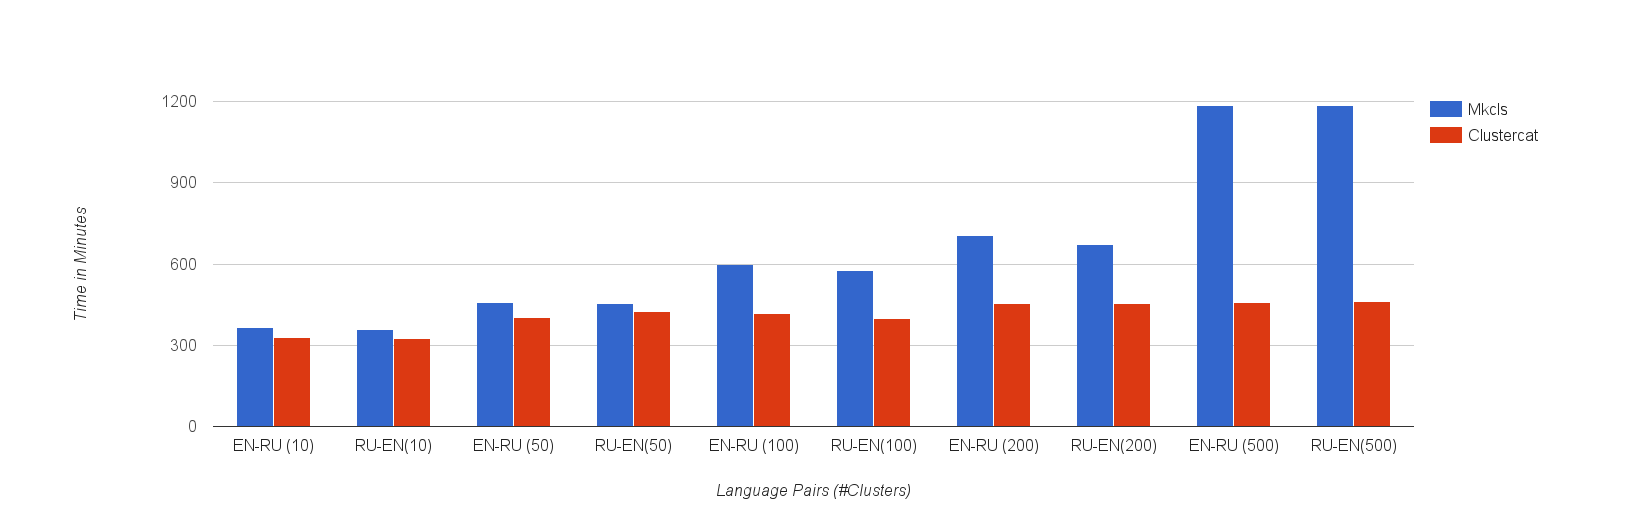
\includegraphics[width=\textwidth]{images/mt-training-times.png} 
	\caption{End-to-end translation model training times for English-Russian and Russian-English for various cluster sizes using \texttt{mkcls} and \texttt{BIRA}.}
	\label{fig-mt-training-times}
\end{figure}

Figure \ref{fig-mt-training-times} shows that \texttt{BIRA} enables MT experiments to explore high cluster sizes without the time-consuming overhead of \texttt{mkcls}. Using the {\tt BIRA} clustering algorithm reduces the translation model training time with 500 clusters from 20 hours using {\tt mkcls} (of which 60\% of the time is spent on clustering) to just 8 hours (of which 5\% is spent on clustering). It takes 8 hours to complete the full translation model training with 500 clusters, as compared to 20 hours using {\tt mkcls}. We bring the time for clustering from 60\% of the total training time to just 5\%\,.This reduces 5\% of the total training time for the {\tt BIRA} clusterer, compared to 60\% for {\tt mkcls}. Using our {\tt BIRA} implementation it takes 9 hours to complete the full translation model training with 1000 clusters, as compared to 30 hours using {\tt mkcls} -- 7\% of the total training time for the {\tt BIRA} clusterer, compared to 74\% for {\tt mkcls}.

\section{Summary}

In this Chapter, we incorporated sub-ontological structures (i.e. word clusters) into machine translation through improving the predictive exchange algorithm that address longstanding drawbacks of the original algorithm compared to other clustering algorithms and showed that word alignment models using the \texttt{BIRA} implementation fully match those using \texttt{mkcls} in BLEU scores, with time savings found by using our improvements.\footnote{The software is freely available at \url{https://github.com/jonsafari/clustercat}.}



